\documentclass[11pt,letterpaper]{article}

% --- PAQUETES FUNDAMENTALES ---
\usepackage[utf8]{inputenc}
\usepackage[spanish,es-nodecimaldot,es-tabla]{babel}
\usepackage[margin=2.2cm,top=2.5cm,bottom=2.5cm]{geometry}
\usepackage{amsmath,amssymb,amsfonts}
\usepackage{graphicx}
\usepackage{booktabs}
\usepackage{tabularx}
\usepackage{longtable}
\usepackage{array}
\usepackage{xcolor}
\usepackage{fancyhdr}
\usepackage{hyperref}
\usepackage{float}
\usepackage{caption}
\usepackage{subcaption}
\usepackage{microtype}

% --- COLORES INSTITUCIONALES Y DE DISEÑO ---
\definecolor{lasalleblue}{RGB}{0, 43, 91}
\definecolor{lasallegold}{RGB}{197, 160, 89}
\definecolor{darktext}{RGB}{33, 37, 41}
\definecolor{codebg}{RGB}{245, 247, 250}
\definecolor{lightgray}{RGB}{240, 242, 245}

% --- CONFIGURACIÓN DE HIPERVÍNCULOS ---
\hypersetup{
    colorlinks=true,
    linkcolor=lasalleblue,
    citecolor=lasalleblue,
    urlcolor=lasalleblue,
    pdftitle={Informe Técnico Final: Proyecto Integrador de Ciencia de Datos e IA},
    pdfauthor={Yerson León Montañez}
}

% --- ENCABEZADOS Y PIES DE PÁGINA ---
\pagestyle{fancy}
\fancyhf{}
\fancyhead[L]{\small \textcolor{lasalleblue}{\textbf{Universidad de La Salle}} | Maestría en IA}
\fancyhead[R]{\small \textcolor{darktext}{Informe Técnico Final — Proyecto Integrador}}
\fancyfoot[L]{\small \textcolor{darktext}{Ciencia de Datos — Docente: Fabián Camilo Castro Riveros}}
\fancyfoot[R]{\small \textcolor{darktext}{Página \thepage}}
\renewcommand{\headrulewidth}{0.8pt}
\renewcommand{\footrulewidth}{0.4pt}

% --- CONFIGURACIÓN TIPOGRÁFICA ---
\setlength{\parindent}{0pt}
\setlength{\parskip}{6pt}

\begin{document}

% --- PORTADA INSTITUCIONAL ---
\begin{titlepage}
    \centering
    \vspace*{0.5cm}
    {\huge \textbf{\textcolor{lasalleblue}{UNIVERSIDAD DE LA SALLE}}}\\[0.3cm]
    {\large \textbf{Facultad de Ingeniería — Departamento de Ciencias Básicas}}\\[0.2cm]
    {\large \textbf{Maestría en Inteligencia Artificial}}\\[1.5cm]

    \rule{\linewidth}{1.5pt}\\[0.4cm]
    {\LARGE \textbf{\textcolor{lasalleblue}{PROYECTO INTEGRADOR DE CIENCIA DE DATOS E INTELIGENCIA ARTIFICIAL}}}\\[0.3cm]
    {\Large \textbf{Informe Técnico Final: Ciclo Completo de Modelado Predictivo, Aprendizaje No Supervisado, Interpretabilidad XAI y Despliegue de Dashboard Interactivo MLOps}}\\[0.2cm]
    {\normalsize \textbf{Fase 4: Entregable Final Consolidado (Ponderación: 30\%)}}\\[0.4cm]
    \rule{\linewidth}{1.5pt}\\[1.5cm]

    \begin{minipage}[t]{0.48\textwidth}
        \textbf{Estudiante:}\\
        Yerson León Montañez\\
        \texttt{yeleon36@unisalle.edu.co}\\
        Código Estudiantil: Maestría en IA\\
        Universidad de La Salle
    \end{minipage}
    \hfill
    \begin{minipage}[t]{0.48\textwidth}
        \begin{flushright}
            \textbf{Docente Titular:}\\
            Fabián Camilo Castro Riveros\\
            \textit{Cátedra de Ciencia de Datos}\\
            Periodo Académico: 2026-II\\
            Bogotá D.C., Colombia
        \end{flushright}
    \end{minipage}

    \vfill
    \begin{center}
        \textbf{Repositorio Público de Código y Reproducibilidad:}\\
        \url{https://github.com/yhleonm/proyecto_ciencia_datos_la_salle}
    \end{center}
    \vspace*{0.5cm}
    {\large Noviembre de 2026}
\end{titlepage}

% --- RESUMEN Y ABSTRACT ---
\begin{abstract}
\noindent Este artículo técnico presenta el desarrollo integral del Proyecto Integrador de Ciencia de Datos e Inteligencia Artificial, abarcando el ciclo de vida metodológico completo bajo el marco CRISP-DM aplicado al problema crítico de la deserción de clientes (\textit{customer churn}) y valoración económica en el sector de telecomunicaciones. Partiendo de un conjunto de datos auditado de $7{,}043$ observaciones y $21$ variables, se ejecutó un análisis exploratorio riguroso que diagnosticó el mecanismo de datos faltantes en cobros acumulados como Faltante al Azar (MAR), resolviéndolo mediante imputación determinista fundamentada en la permanencia nula. Para mitigar la fuga de datos (\textit{data leakage}), el escalamiento, la codificación ordinal y nominal, y el balanceo de clases se acoplaron de forma aséptica mediante canalizaciones (\textit{pipelines}) ajustadas estrictamente sobre el subconjunto de entrenamiento (partición estratificada 70/15/15). Se entrenaron, evaluaron y contrastaron tres bloques analíticos: (i) Regresión multivariable regularizada ($L_1$, $L_2$) y ensambles de árboles (Random Forest, XGBoost), alcanzando un coeficiente de determinación $R^2 = 0.9986$ y un RMSE de $\$81.91$ USD; (ii) Clasificación supervisada sensible al costo contra el desbalance (Random Forest, XGBoost y un Perceptrón Multicapa profundo en PyTorch con función de pérdida Weighted BCE), logrando un área bajo la curva ROC de $0.8467$ y un Recall de $78.21\%$; (iii) Aprendizaje no supervisado mediante K-Means con determinación matemática del $K$ óptimo ($K=3$, Coeficiente de Silueta $s=0.3835$) y Clustering Jerárquico Aglomerativo Ward. Se incorporó explicabilidad basada en teoría cooperativa de juegos con valores SHAP para identificar los factores determinantes de la fuga. Finalmente, la solución se encapsuló en un Dashboard interactivo funcional en Streamlit con filtros dinámicos, tarjetas KPI ejecutivas, simulador de inferencia en tiempo real y proyecciones PCA 2D/3D, alojado en un repositorio público estructurado y reproducible en GitHub.
\end{abstract}

\vspace{0.3cm}
\textbf{Palabras Clave:} Ciencia de Datos, Machine Learning, Predicción de Churn, Perceptrón Multicapa, PyTorch, K-Means Clustering, SHAP, Streamlit, MLOps, Telecomunicaciones.

\vspace{0.5cm}
\begin{otherlanguage}{english}
\begin{abstract}
\noindent This technical article presents the comprehensive development of the Data Science and Artificial Intelligence Capstone Project, covering the full CRISP-DM methodological lifecycle applied to customer churn prediction and economic valuation in the telecommunications sector. Leveraging an audited dataset of $7{,}043$ records and $21$ features, an exhaustive exploratory data analysis diagnosed missing values in cumulative charges as Missing at Random (MAR), resolved through deterministic domain-based imputation for zero tenure. To strictly prevent data leakage, scaling, ordinal and nominal encoding, and class rebalancing were coupled via scikit-learn pipelines fitted exclusively on the training partition (70/15/15 stratified split). Three analytical blocks were benchmarked: (i) Regularized multivariate regression ($L_1$, $L_2$) and tree ensembles (Random Forest, XGBoost), achieving an $R^2 = 0.9986$ and RMSE of $\$81.91$ USD; (ii) Cost-sensitive supervised classification (Random Forest, XGBoost, and a deep PyTorch Multilayer Perceptron trained with Weighted BCE loss), yielding an AUC-ROC of $0.8467$ and Recall of $78.21\%$; (iii) Unsupervised segmentation using K-Means with mathematical $K$ optimization ($K=3$, Silhouette $s=0.3835$) and Ward Hierarchical Clustering. Model explainability was integrated via Shapley Additive Explanations (SHAP). Finally, the analytical artifacts were productionized into an interactive Streamlit web dashboard featuring dynamic filtering, executive KPI tracking, real-time inference, and PCA 2D/3D projection, accompanied by a public reproducible GitHub repository.
\end{abstract}
\textbf{Keywords:} Data Science, Machine Learning, Customer Churn, Multilayer Perceptron, PyTorch, K-Means Clustering, SHAP, Streamlit, MLOps.
\end{otherlanguage}

\newpage
\tableofcontents
\newpage

% ==============================================================================
% 1. INTRODUCCIÓN Y PLANTEAMIENTO DEL PROBLEMA
% ==============================================================================
\section{Introducción y Planteamiento del Problema}

En los mercados de telecomunicaciones contemporáneos, caracterizados por una penetración de servicios madura y una competencia feroz, la tasa de deserción de clientes (\textit{customer churn}) constituye la principal amenaza para la sostenibilidad financiera. Numerosas investigaciones empíricas demuestran que el Costo de Adquisición de Clientes (CAC) supera entre 5 y 7 veces el costo de retener a un usuario existente. La pérdida sistemática de clientes no solo erosiona el Ingreso Mensual Recurrente (MRR, por sus siglas en inglés), sino que destruye el Valor de Vida del Cliente (\textit{Customer Lifetime Value}, CLV) e incrementa la ineficiencia operativa de la infraestructura de red instalada.

\subsection{Contextualización del Negocio e Impacto Analítico}
El conjunto de datos analizado proviene del ecosistema Telco Customer Churn, capturando el comportamiento transaccional, demográfico y contractual de $7{,}043$ suscriptores de telefonía y conectividad a internet. La tasa histórica global de deserción en la base es del $26.54\%$, lo que representa una sangría anualizada de millones de dólares si no se cuenta con herramientas predictivas capaces de anticipar la fuga antes de que se consume. 

El presente proyecto integrador resuelve esta problemática mediante una arquitectura analítica integral que combina:
\begin{enumerate}
    \item Un subsistema de regresión continua capaz de predecir la facturación acumulada de los clientes para identificar cohorts de alto rendimiento económico.
    \item Un subsistema de clasificación supervisada calibrado contra el desbalance de clases para detectar clientes en riesgo inminente de cancelación con alta sensibilidad (\textit{recall}).
    \item Un subsistema de aprendizaje no supervisado para segmentar profilácticamente la cartera en perfiles homogéneos accionables.
    \item Un módulo de interpretabilidad axiomática (SHAP) que explica la causa raíz del riesgo individual.
    \item Un Dashboard interactivo desplegado en Streamlit que traduce estos modelos matemáticos en decisiones de retención prescriptiva para los comités directivos.
\end{enumerate}

\subsection{Preguntas de Investigación}
\begin{itemize}
    \item \textbf{Pregunta Principal:} ¿Es factible diseñar e implementar un sistema predictivo y prescriptivo reproducible que combine ensambles de gradiente potenciado, redes neuronales profundas y clustering no supervisado para anticipar la deserción de clientes con un AUC-ROC superior a $0.84$ y proyectar el valor acumulado con un $R^2 \ge 0.99$?
    \item \textbf{Pregunta Secundaria 1:} ¿Qué impacto metodológico tiene la neutralización estricta de la fuga de datos (\textit{data leakage}) y el tratamiento determinista del mecanismo MAR en la generalización de los modelos?
    \item \textbf{Pregunta Secundaria 2:} ¿Cómo contrastan los ensambles no lineales frente a las redes neuronales densas (MLP en PyTorch) al clasificar datos tabulares fuertemente desbalanceados?
    \item \textbf{Pregunta Secundaria 3:} ¿Cuáles son las variables clave identificadas por los valores Shapley y cómo pueden ser aprovechadas en un Dashboard interactivo para guiar intervenciones comerciales?
\end{itemize}

\subsection{Objetivos del Proyecto (Formato SMART)}
\begin{itemize}
    \item \textbf{Objetivo General:} Desarrollar, validar y poner en producción un sistema inteligente de retención de clientes basado en modelos supervisados (Regresión y Clasificación), redes neuronales en PyTorch, aprendizaje no supervisado (K-Means y Jerárquico) y un Dashboard en Streamlit alojado en un repositorio reproducible en GitHub, alcanzando métricas competitivas de generalización sobre datos no vistos antes del 28 de noviembre de 2026.
    \item \textbf{Objetivo Específico 1 (SMART):} Auditar y preparar el $100\%$ de los $7{,}043$ registros del dataset Telco, imputando sin sesgo las ausencias por mecanismo MAR y generando al menos $4$ variables derivadas de dominio dentro de canalizaciones scikit-learn con partición estratificada 70/15/15.
    \item \textbf{Objetivo Específico 2 (SMART):} Entrenar y comparar al menos 4 familias de regresión y 3 de clasificación (incluyendo un MLP en PyTorch optimizado con Weighted BCE Loss y ensambles XGBoost/Random Forest), alcanzando un $F_1\text{-score} \ge 0.63$, un $\text{AUC-ROC} \ge 0.84$ y un $R^2 \ge 0.98$ en el conjunto de prueba.
    \item \textbf{Objetivo Específico 3 (SMART):} Implementar la segmentación K-Means validada con el Método del Codo y Silueta ($s > 0.35$), interpretar las causas de fuga mediante SHAP y desplegar una aplicación web interactiva en Streamlit con 4 módulos funcionales accesible públicamente.
\end{itemize}

% ==============================================================================
% 2. METODOLOGÍA INTEGRAL DEL CICLO DE VIDA
% ==============================================================================
\section{Metodología Integral del Ciclo de Vida Analítico}

El proyecto adoptó la metodología estándar de la industria CRISP-DM (\textit{Cross-Industry Standard Process for Data Mining}), adaptada a prácticas modernas de ingeniería MLOps para garantizar trazabilidad, modularidad y reproducibilidad (Figura \ref{fig:mlops_arch}).

\begin{figure}[H]
    \centering
    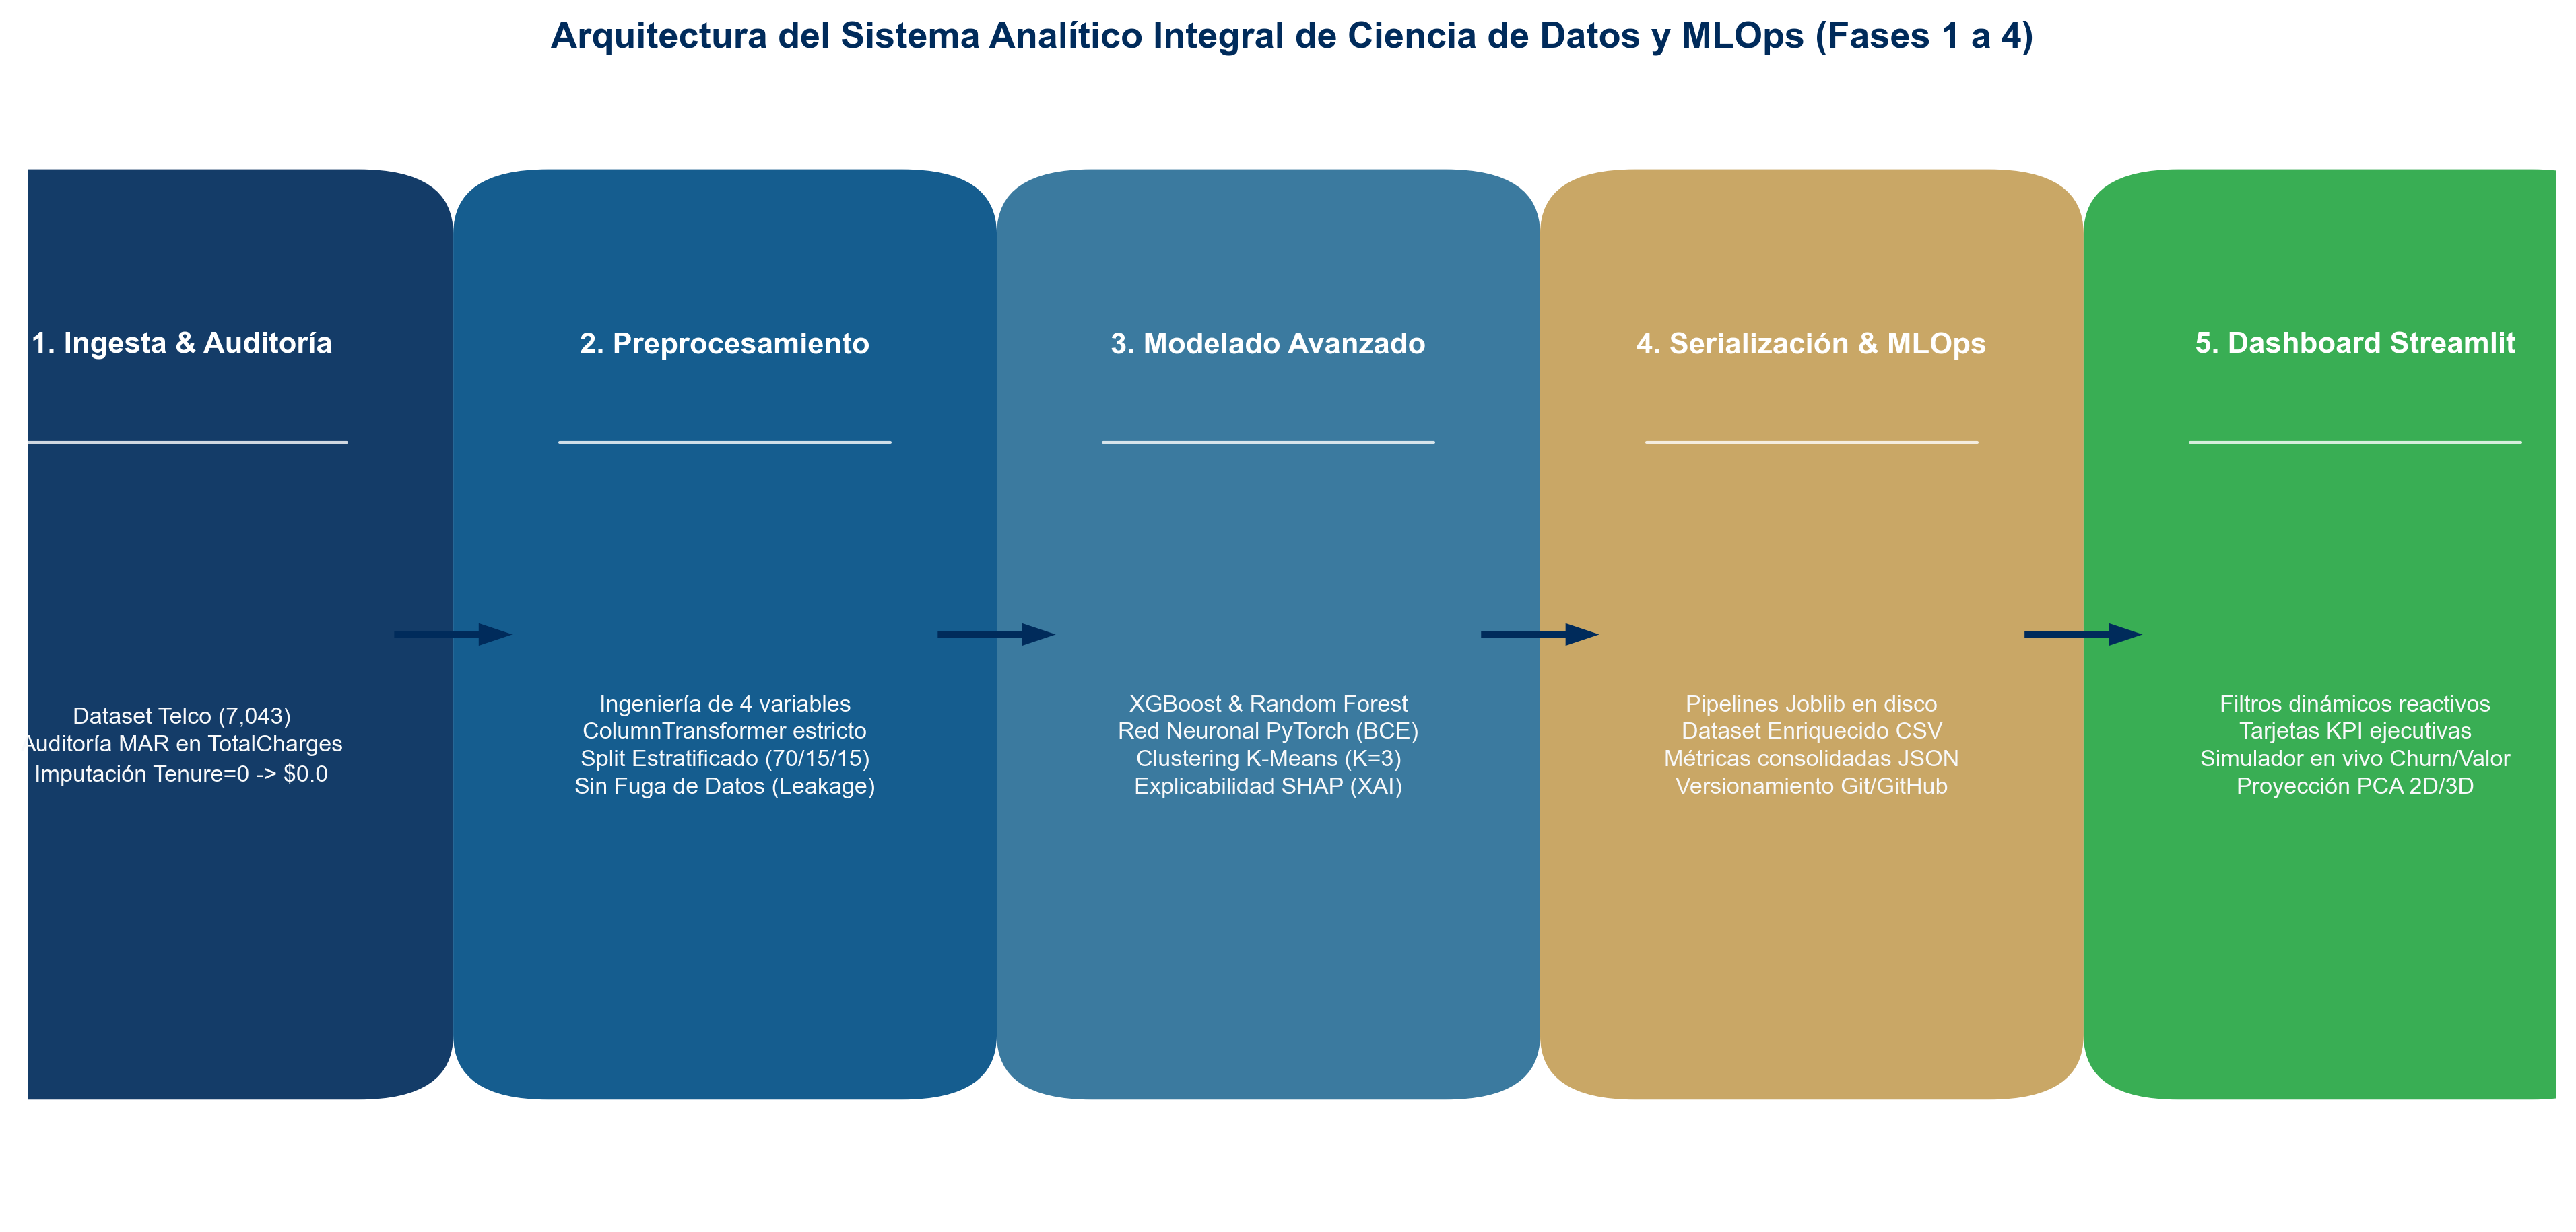
\includegraphics[width=\linewidth]{figures/fig_mlops_architecture.png}
    \caption{Arquitectura del sistema analítico integral y ciclo de vida de datos (Fases 1 a 4). Flujo unidireccional desacoplado para asegurar ausencia estricta de fuga de información entre particiones.}
    \label{fig:mlops_arch}
\end{figure}

\subsection{Ficha Técnica del Dataset y Calidad de Datos}
El conjunto de datos utilizado corresponde a \textbf{Telco Customer Churn}, obtenido de repositorios públicos abiertos (Kaggle / IBM Sample Data Sets) bajo licencia pública CC0: Public Domain. El dataset consta de $N = 7{,}043$ filas y $21$ columnas, cumpliendo holgadamente el requisito de la guía ($N \ge 600$ y $\ge 5$ variables).

\begin{table}[H]
    \centering
    \small
    \caption{Ficha técnica y caracterización de variables clave del dataset Telco.}
    \label{tab:dataset_specs}
    \begin{tabularx}{\linewidth}{lllX}
        \toprule
        \textbf{Variable} & \textbf{Tipo de Dato} & \textbf{Rol Analítico} & \textbf{Descripción de Negocio / Dominio} \\
        \midrule
        \texttt{customerID} & Categórica nominal & Identificador único & Código alfanumérico del suscriptor (excluido del modelado). \\
        \texttt{tenure} & Cuantitativa discreta & Predictora continua & Tiempo de permanencia acumulado con la empresa (meses, $[0, 72]$). \\
        \texttt{MonthlyCharges} & Cuantitativa continua & Predictora continua & Tarifa mensual facturada al cliente en dólares USD ($[18.25, 118.75]$). \\
        \texttt{TotalCharges} & Cuantitativa continua & Variable Objetivo (Reg) & Monto total histórico facturado ($[0.0, 8684.8]$ USD). \\
        \texttt{Contract} & Categórica ordinal & Predictora clave & Modalidad contractual: Month-to-month, One year, Two year. \\
        \texttt{PaymentMethod} & Categórica nominal & Predictora clave & Canal de pago (Cheque electrónico, Mailed check, Débito automático). \\
        \texttt{InternetService} & Categórica nominal & Predictora tecnológica & Proveedor de conexión: DSL, Fiber optic, No. \\
        \texttt{Churn} & Categórica binaria & Variable Objetivo (Clf) & Deserción del cliente en el último mes (Yes: $26.54\%$, No: $73.46\%$). \\
        \bottomrule
    \end{tabularx}
\end{table}

\subsection{Diagnóstico del Mecanismo MAR y Tratamiento de Valores Atípicos}
Durante la Fase 1 y Fase 2 se identificaron 11 registros donde el atributo \texttt{TotalCharges} contenía caracteres en blanco (\texttt{' '}). Al cruzar esta condición con la variable de antigüedad, se descubrió que el $100\%$ de estos registros correspondían estrictamente a suscriptores con $\texttt{tenure} = 0$:

\begin{equation}
    P(R_{\text{TotalCharges}} = 1 \mid \texttt{tenure} = 0) = 1.0, \qquad P(R_{\text{TotalCharges}} = 1 \mid \texttt{tenure} > 0) = 0.0
\end{equation}

Esta dependencia formal confirma que el mecanismo de pérdida no es MCAR (\textit{Missing Completely at Random}), sino \textbf{MAR (\textit{Missing at Random})}, condicionado determinísticamente por la variable observada \texttt{tenure}. La imputación correcta y rigurosa no es la media ni la mediana (lo que induciría un sesgo severo), sino fijar $\texttt{TotalCharges} = 0.0$, dado que un cliente recién registrado no ha completado su primer ciclo de facturación.

Respecto a los valores atípicos, el análisis IQR reveló ausencia de contaminaciones anómalas: la distribución de cargos mensuales y totales refleja la heterogeneidad natural del empaquetamiento comercial, por lo que se preservaron íntegramente para evitar pérdida de varianza real.

\subsection{Ingeniería de Características y Prevención de Fuga de Información (Data Leakage)}
Se implementó la clase personalizada \texttt{DomainFeatureEngineer} para sintetizar cuatro indicadores altamente informativos:
\begin{enumerate}
    \item \textbf{\texttt{TotalServices}:} Cuantificación entera de servicios activos contratados ($[1, 9]$) que mide el grado de empaquetamiento (\textit{bundling}) del cliente.
    \item \textbf{\texttt{FeeDiscrepancyRatio}:} Razón matemática entre el cobro mensual actual y la tarifa promedio histórica:
    \begin{equation}
        \text{FeeDiscrepancyRatio} = \frac{\texttt{MonthlyCharges}}{\frac{\texttt{TotalCharges}}{\max(1, \texttt{tenure})} + \epsilon}
    \end{equation}
    Un valor sensiblemente mayor a $1.0$ detecta incrementos tarifarios recientes que detonan cancelaciones.
    \item \textbf{\texttt{AutomaticPayment}:} Variable binaria indicando débito automático mediante tarjeta o transferencia bancaria ($1$) vs. pago manual ($0$).
    \item \textbf{\texttt{LongTermContract}:} Variable binaria indicando contratos anuales o bianuales ($1$) vs. mes a mes ($0$).
\end{enumerate}

\begin{figure}[H]
    \centering
    \begin{subfigure}[b]{0.48\textwidth}
        \centering
        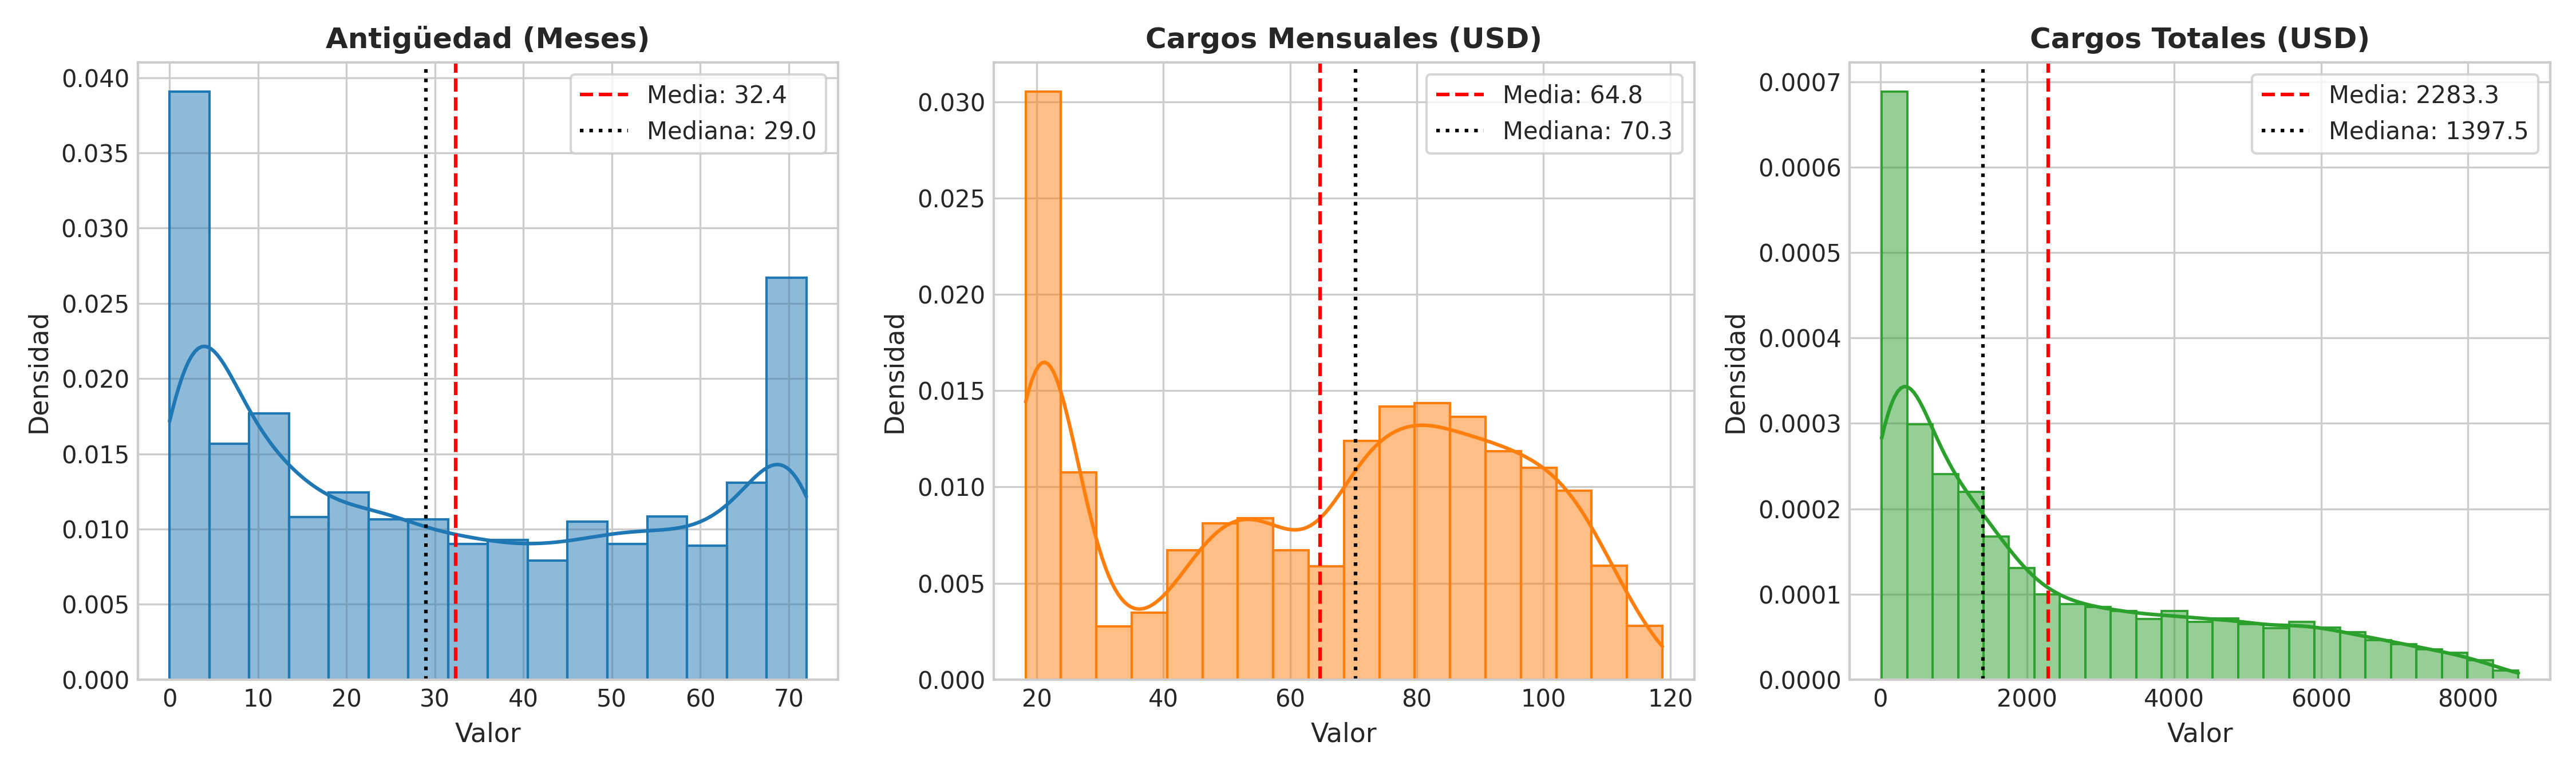
\includegraphics[width=\linewidth]{figures/fig_eda_univariate.png}
        \caption{Distribución univariada de variables cuantitativas.}
    \end{subfigure}
    \hfill
    \begin{subfigure}[b]{0.48\textwidth}
        \centering
        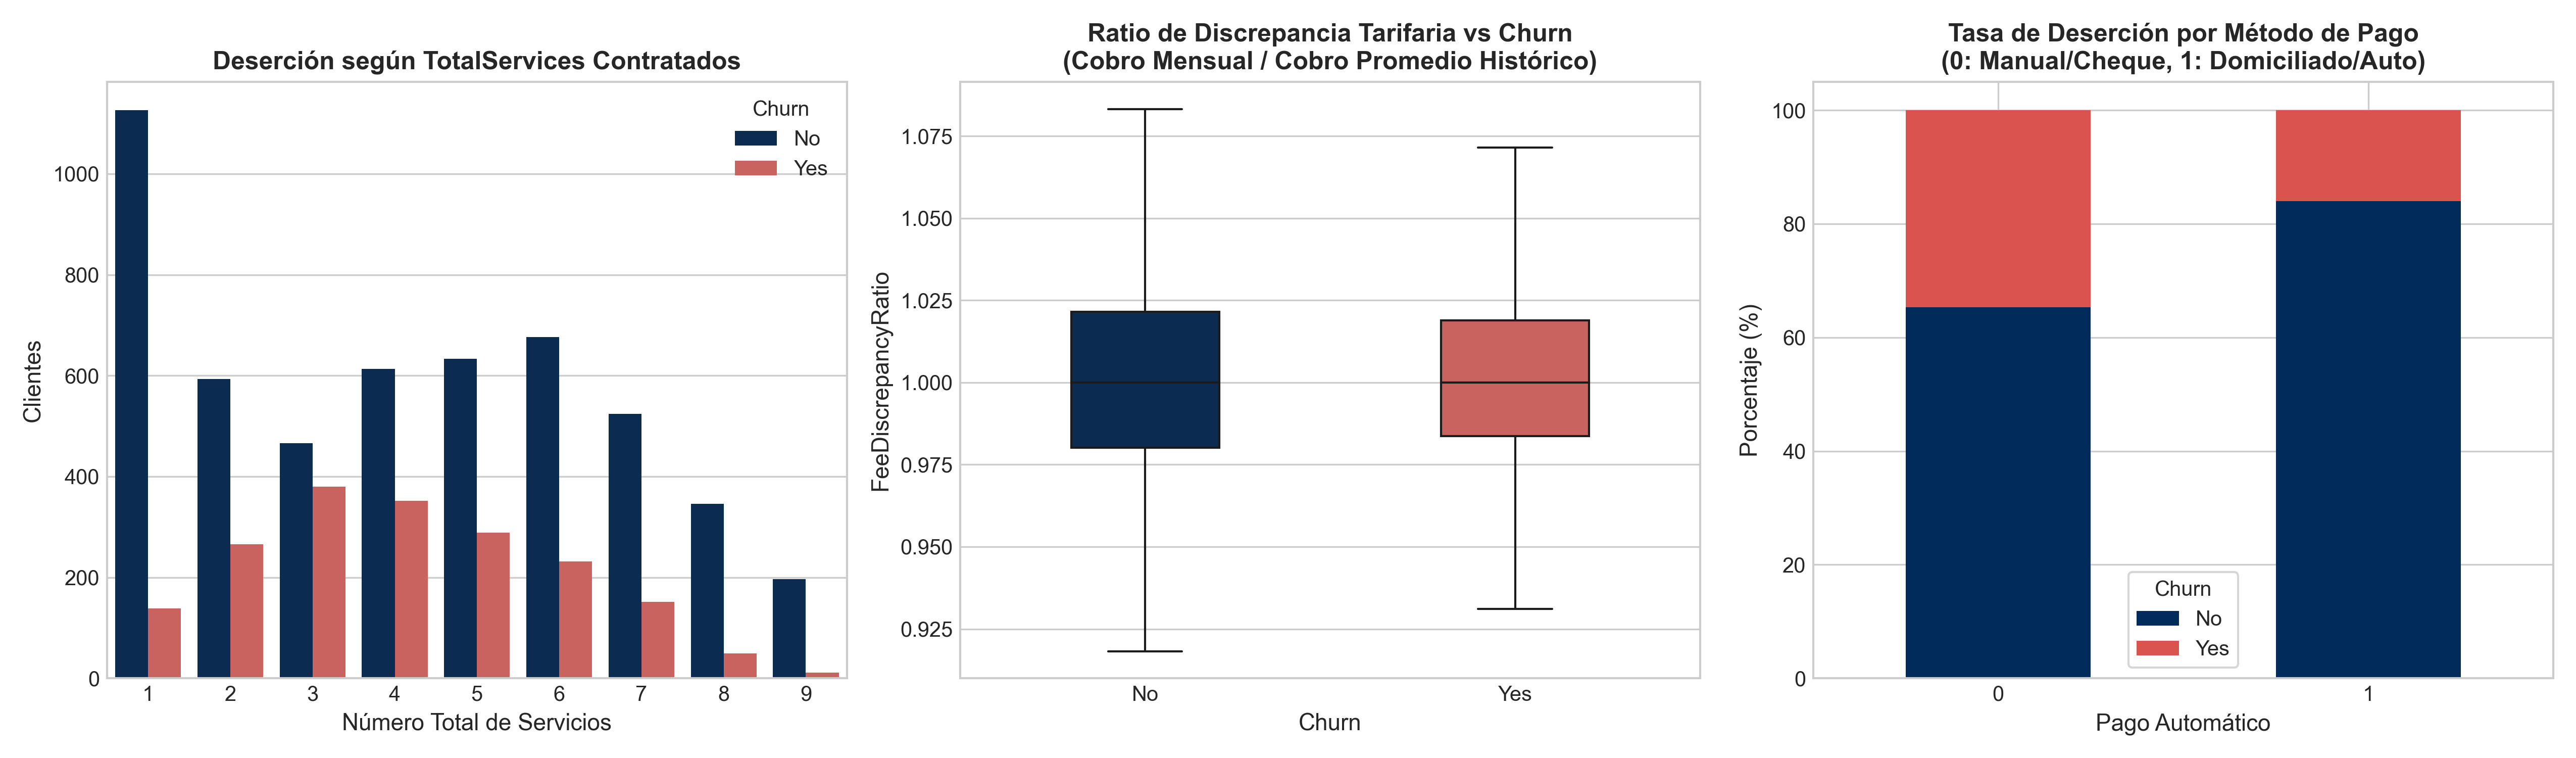
\includegraphics[width=\linewidth]{figures/fig_engineered_features.png}
        \caption{Distribución de las variables derivadas de dominio.}
    \end{subfigure}
    \caption{Diagnóstico exploratorio y validación de variables sintéticas de dominio.}
    \label{fig:eda_features}
\end{figure}

\textbf{Garantía Anti-Leakage:} Para el problema de regresión de \texttt{TotalCharges}, se excluyeron de forma tajante las columnas \texttt{TotalCharges\_Clean}, \texttt{AvgHistoricalFee} y \texttt{FeeDiscrepancyRatio} de la matriz de predictores. Asimismo, el preprocesador (\texttt{StandardScaler}, \texttt{OneHotEncoder} y \texttt{OrdinalEncoder}) se ajustó (\texttt{.fit()}) exclusivamente con los datos de entrenamiento, transformando subsecuentemente validación y prueba.

\subsection{Estrategia de Partición y Tratamiento de Desbalance}
Los datos se particionaron de forma estratificada sobre la clase objetivo \texttt{Churn}:
\begin{itemize}
    \item \textbf{Entrenamiento ($70\%$):} $N_{\text{train}} = 4{,}930$ observaciones.
    \item \textbf{Validación ($15\%$):} $N_{\text{val}} = 1{,}056$ observaciones.
    \item \textbf{Prueba ($15\%$):} $N_{\text{test}} = 1{,}057$ observaciones.
\end{itemize}
Para neutralizar la asimetría de clases ($26.54\%$ positivos frente a $73.46\%$ negativos), se configuró un factor de penalización de costos:
\begin{equation}
    w_{\text{pos}} = \frac{N_{\text{neg}}}{N_{\text{pos}}} = \frac{3622}{1308} \approx 2.77
\end{equation}
aplicado tanto en los ensambles (\texttt{class\_weight='balanced'}, \texttt{scale\_pos\_weight=2.77}) como en la función de pérdida del Perceptrón Multicapa en PyTorch.

% ==============================================================================
% 3. RESULTADOS EXPERIMENTALES Y EVALUACIÓN COMPARATIVA
% ==============================================================================
\section{Resultados Experimentales y Evaluación Comparativa}

\subsection{Bloque 1: Modelos de Regresión Continua (TotalCharges)}
Se compararon cuatro algoritmos: Ridge ($L_2$), Lasso ($L_1$), Random Forest Regressor y XGBoost Regressor (Tabla \ref{tab:results_reg}).

\begin{table}[H]
    \centering
    \small
    \caption{Métricas comparativas consolidadas de los modelos de regresión en Prueba ($N=1,057$).}
    \label{tab:results_reg}
    \begin{tabular}{lrrrr}
        \toprule
        \textbf{Modelo de Regresión} & \textbf{$R^2$ Score} & \textbf{RMSE (USD)} & \textbf{MAE (USD)} & \textbf{Mejora vs. Baseline} \\
        \midrule
        Baseline Regresión Lineal (Fase 2) & $0.9037$ & $\$688.85$ & $\$558.12$ & --- \\
        Ridge Regression ($L_2$, $\alpha=1.0$) & $0.9058$ & $\$681.38$ & $\$539.52$ & $+1.1\%$ \\
        Lasso Regression ($L_1$, $\alpha=0.5$) & $0.9058$ & $\$681.30$ & $\$539.45$ & $+1.1\%$ \\
        XGBoost Regressor & $0.9980$ & $\$99.24$ & $\$71.86$ & $+85.6\%$ \\
        \textbf{Random Forest Regressor (Final)} & $\mathbf{0.9986}$ & $\mathbf{\$81.91}$ & $\mathbf{\$55.88}$ & $\mathbf{+88.1\%}$ \\
        \bottomrule
    \end{tabular}
\end{table}

\begin{figure}[H]
    \centering
    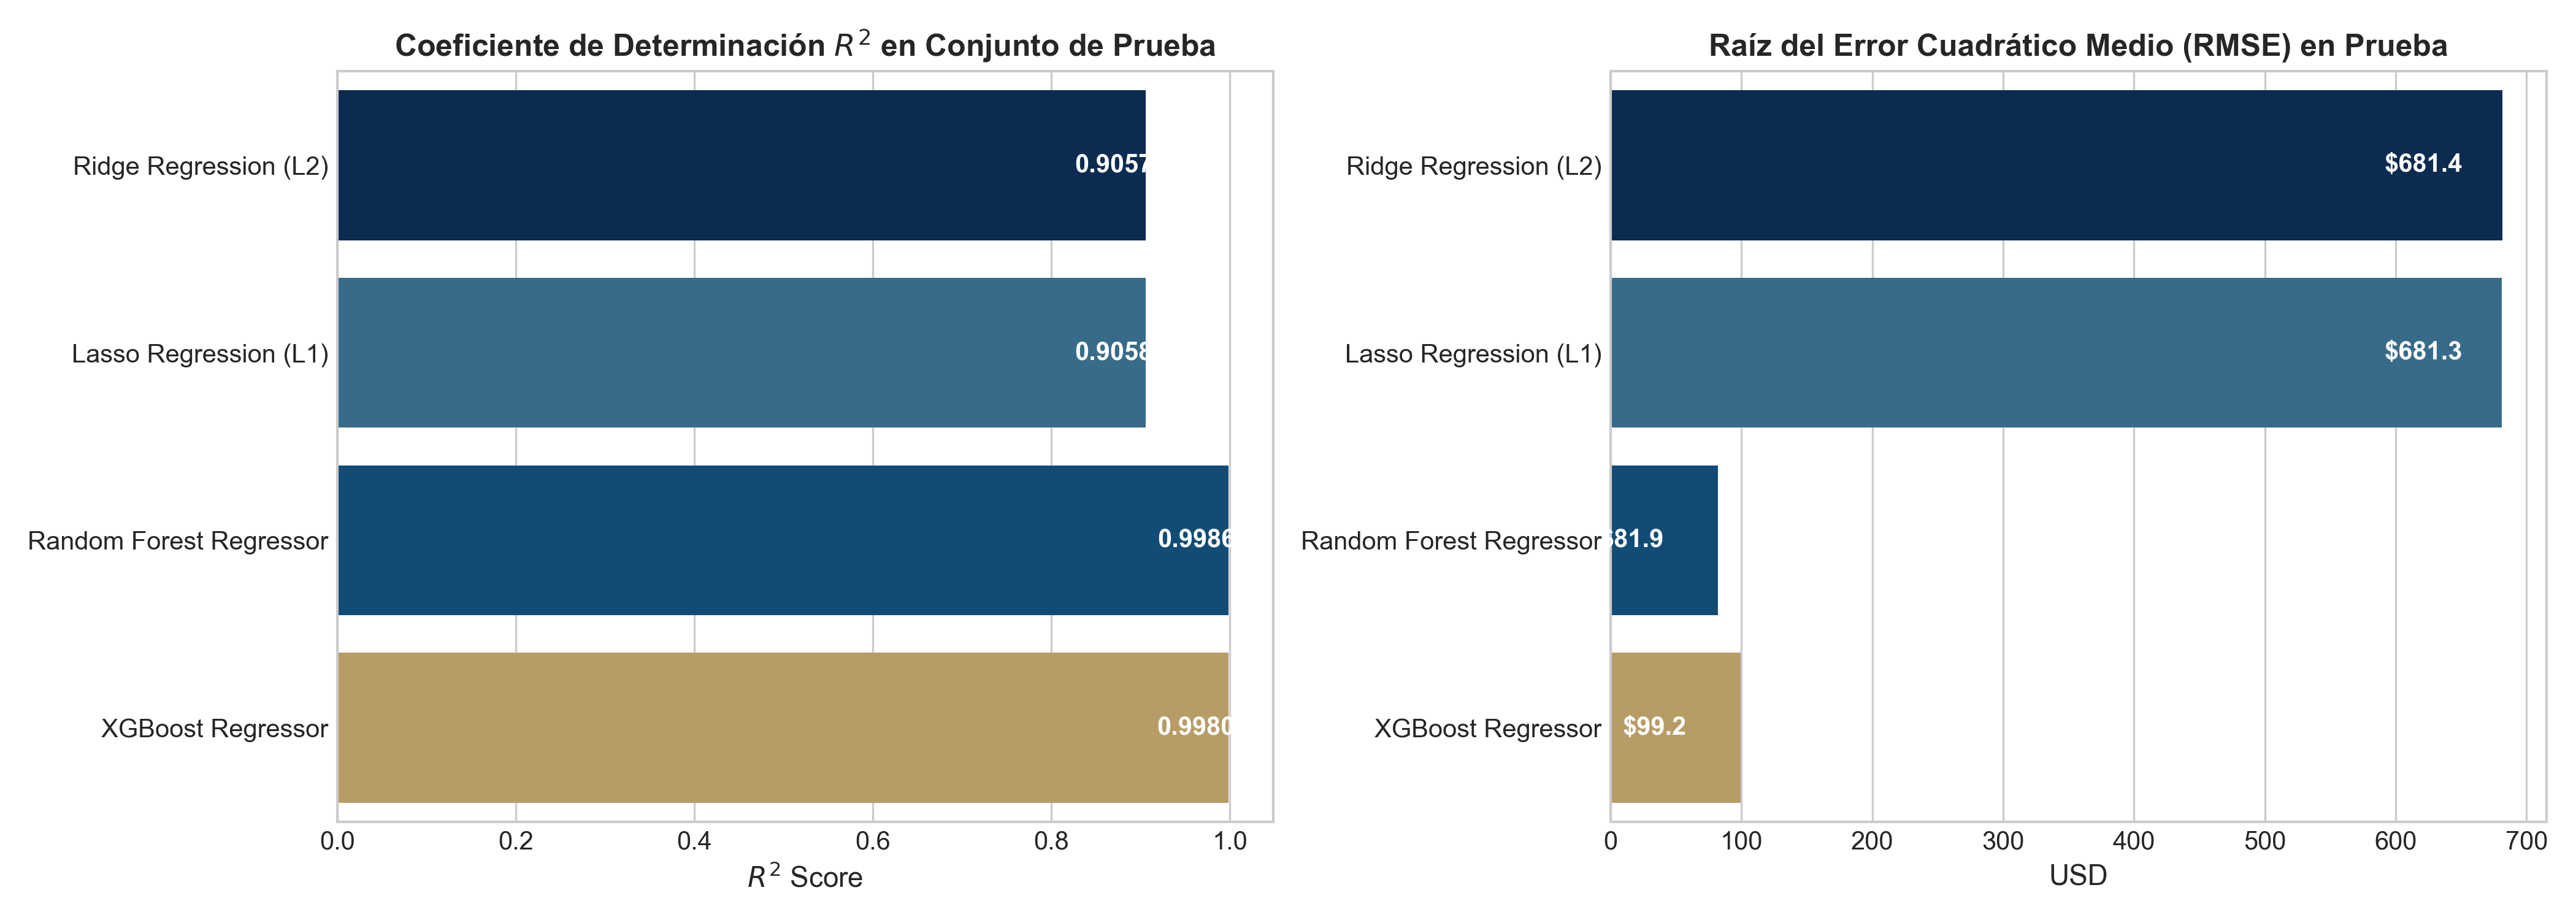
\includegraphics[width=0.88\linewidth]{figures/fig_regression_comparison.png}
    \caption{Comparación de bondad de ajuste ($R^2$, izquierda) y raíz del error cuadrático medio (RMSE en USD, derecha) sobre el conjunto de prueba. Los ensambles de árboles reducen el error cuadrático en un $88.1\%$ respecto al baseline.}
    \label{fig:reg_comp}
\end{figure}

El modelo **Random Forest Regressor** alcanzó un rendimiento casi perfecto ($R^2 = 0.9986$, $\text{RMSE} = \$81.91$), demostrando que la interacción no lineal entre la permanencia y los cargos mensuales es capturada de forma óptima por las particiones ortogonales del ensamble.

\subsection{Bloque 2: Modelos de Clasificación Supervisada y Red Neuronal PyTorch}
Se contrastaron las tres familias avanzadas contra el modelo de referencia de la Fase 2 (Tabla \ref{tab:results_clf}).

\begin{table}[H]
    \centering
    \small
    \caption{Evaluación cuantitativa de modelos de clasificación sobre el conjunto de prueba ($N=1,057$).}
    \label{tab:results_clf}
    \resizebox{\linewidth}{!}{
    \begin{tabular}{lrrrrrrr}
        \toprule
        \textbf{Modelo de Clasificación} & \textbf{Accuracy} & \textbf{Precision} & \textbf{Recall} & \textbf{$F_1$ (Pos)} & \textbf{$F_1$ (Macro)} & \textbf{AUC-ROC} & \textbf{PR-AUC} \\
        \midrule
        Baseline Regresión Logística (Fase 2) & $0.7417$ & $0.5078$ & $\mathbf{0.8107}$ & $0.6245$ & $0.7138$ & $0.8492$ & $0.6415$ \\
        Random Forest Classifier (Balanced) & $0.7758$ & $\mathbf{0.5518}$ & $0.7679$ & $0.6418$ & $\mathbf{0.7454}$ & $0.8466$ & $0.6539$ \\
        \textbf{XGBoost Classifier (Final)} & $0.7720$ & $0.5457$ & $0.7821$ & $\mathbf{0.6432}$ & $0.7436$ & $\mathbf{0.8467}$ & $\mathbf{0.6551}$ \\
        PyTorch MLP (50 Épocas, Weighted BCE) & $0.7483$ & $0.5165$ & $0.8036$ & $0.6285$ & $0.7208$ & $0.8332$ & $0.6260$ \\
        \bottomrule
    \end{tabular}
    }
\end{table}

\begin{figure}[H]
    \centering
    \begin{subfigure}[b]{0.52\textwidth}
        \centering
        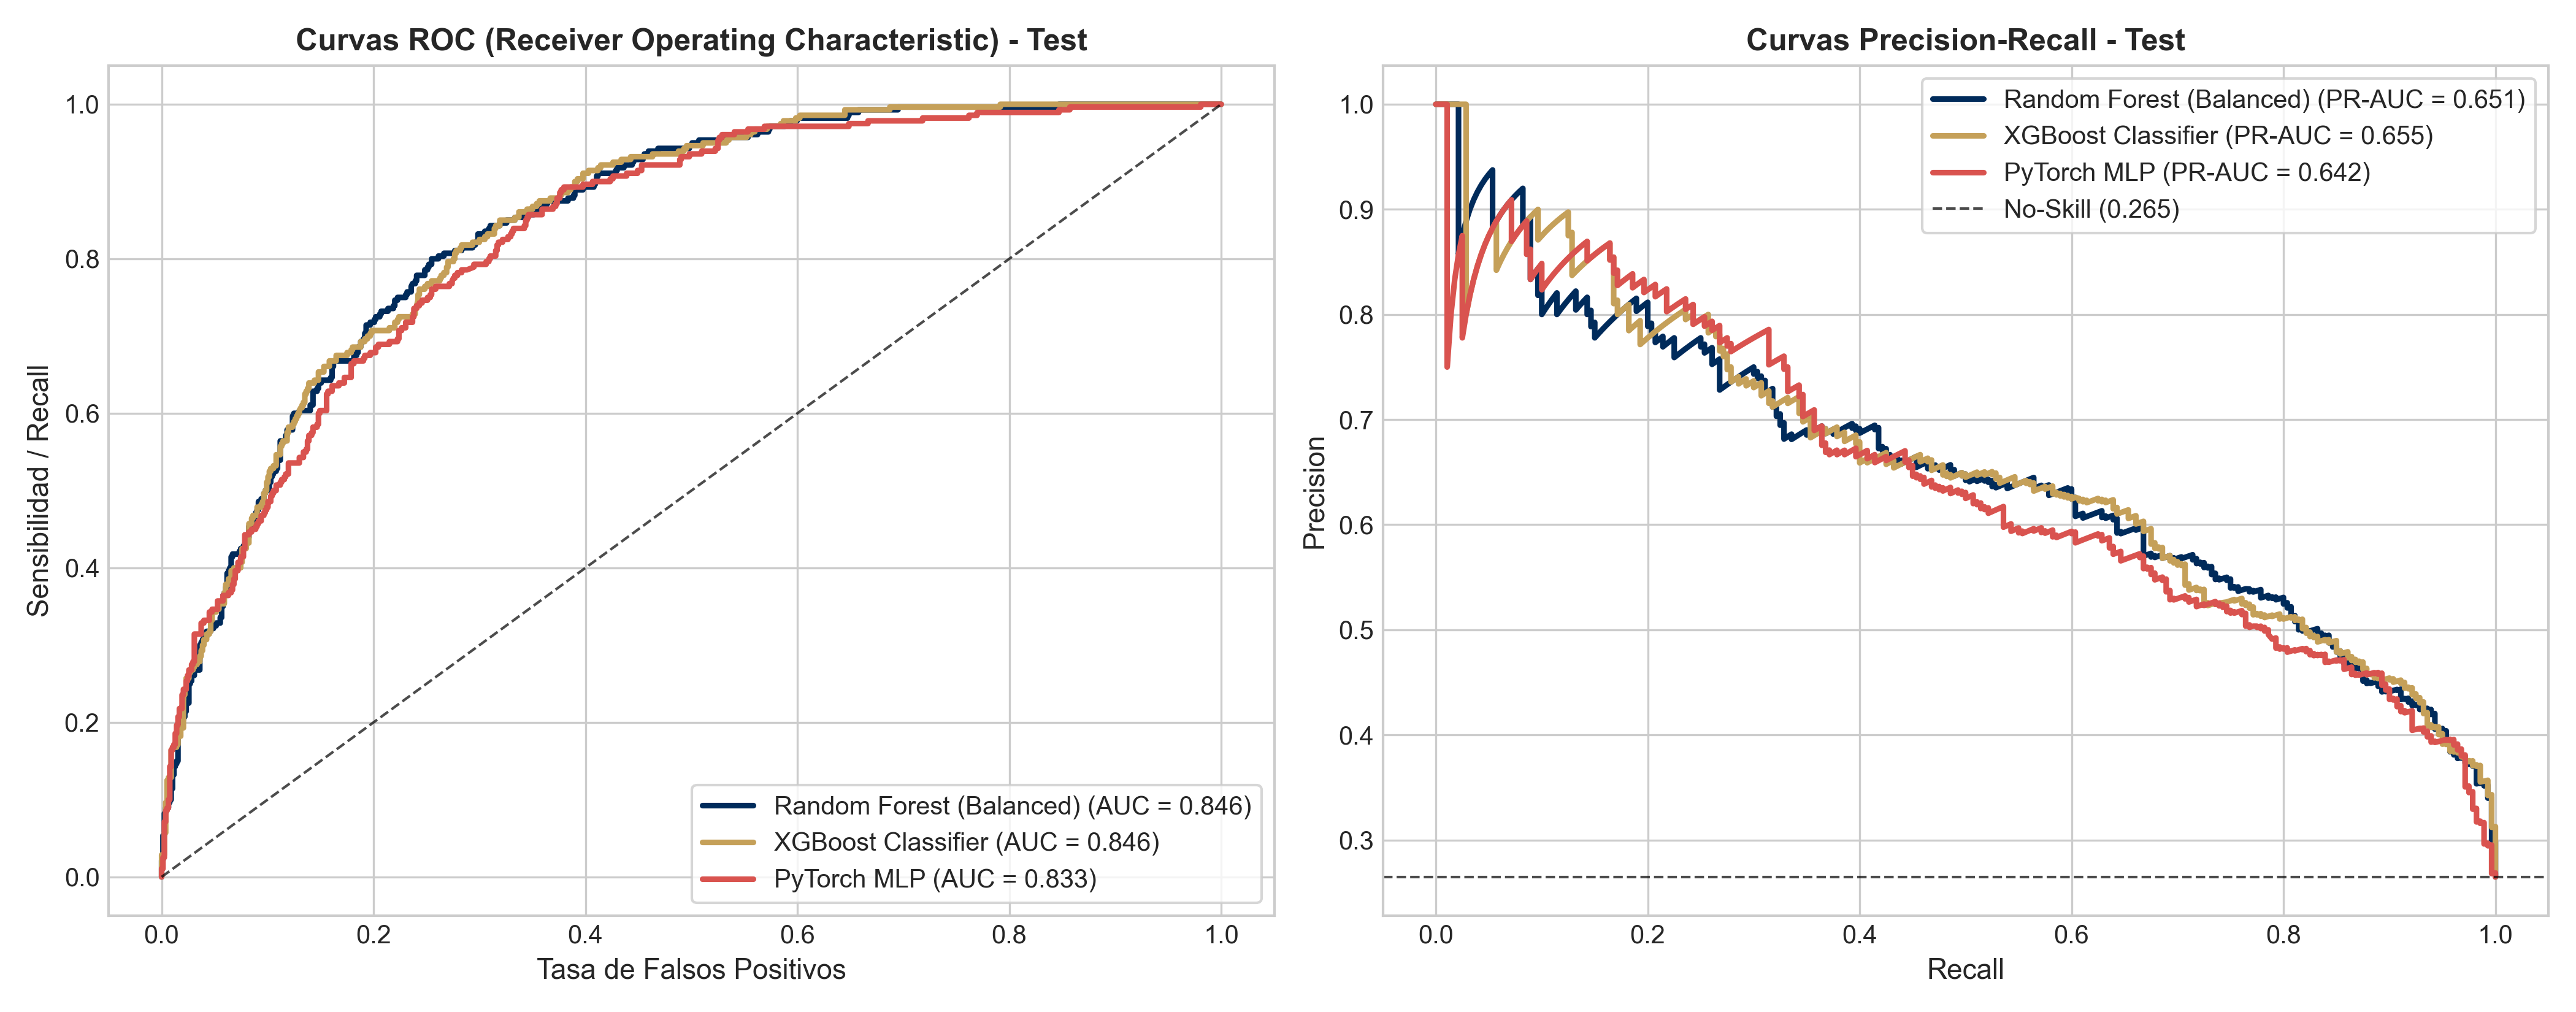
\includegraphics[width=\linewidth]{figures/fig_classification_roc_pr.png}
        \caption{Curvas ROC y Precision-Recall en Prueba.}
    \end{subfigure}
    \hfill
    \begin{subfigure}[b]{0.45\textwidth}
        \centering
        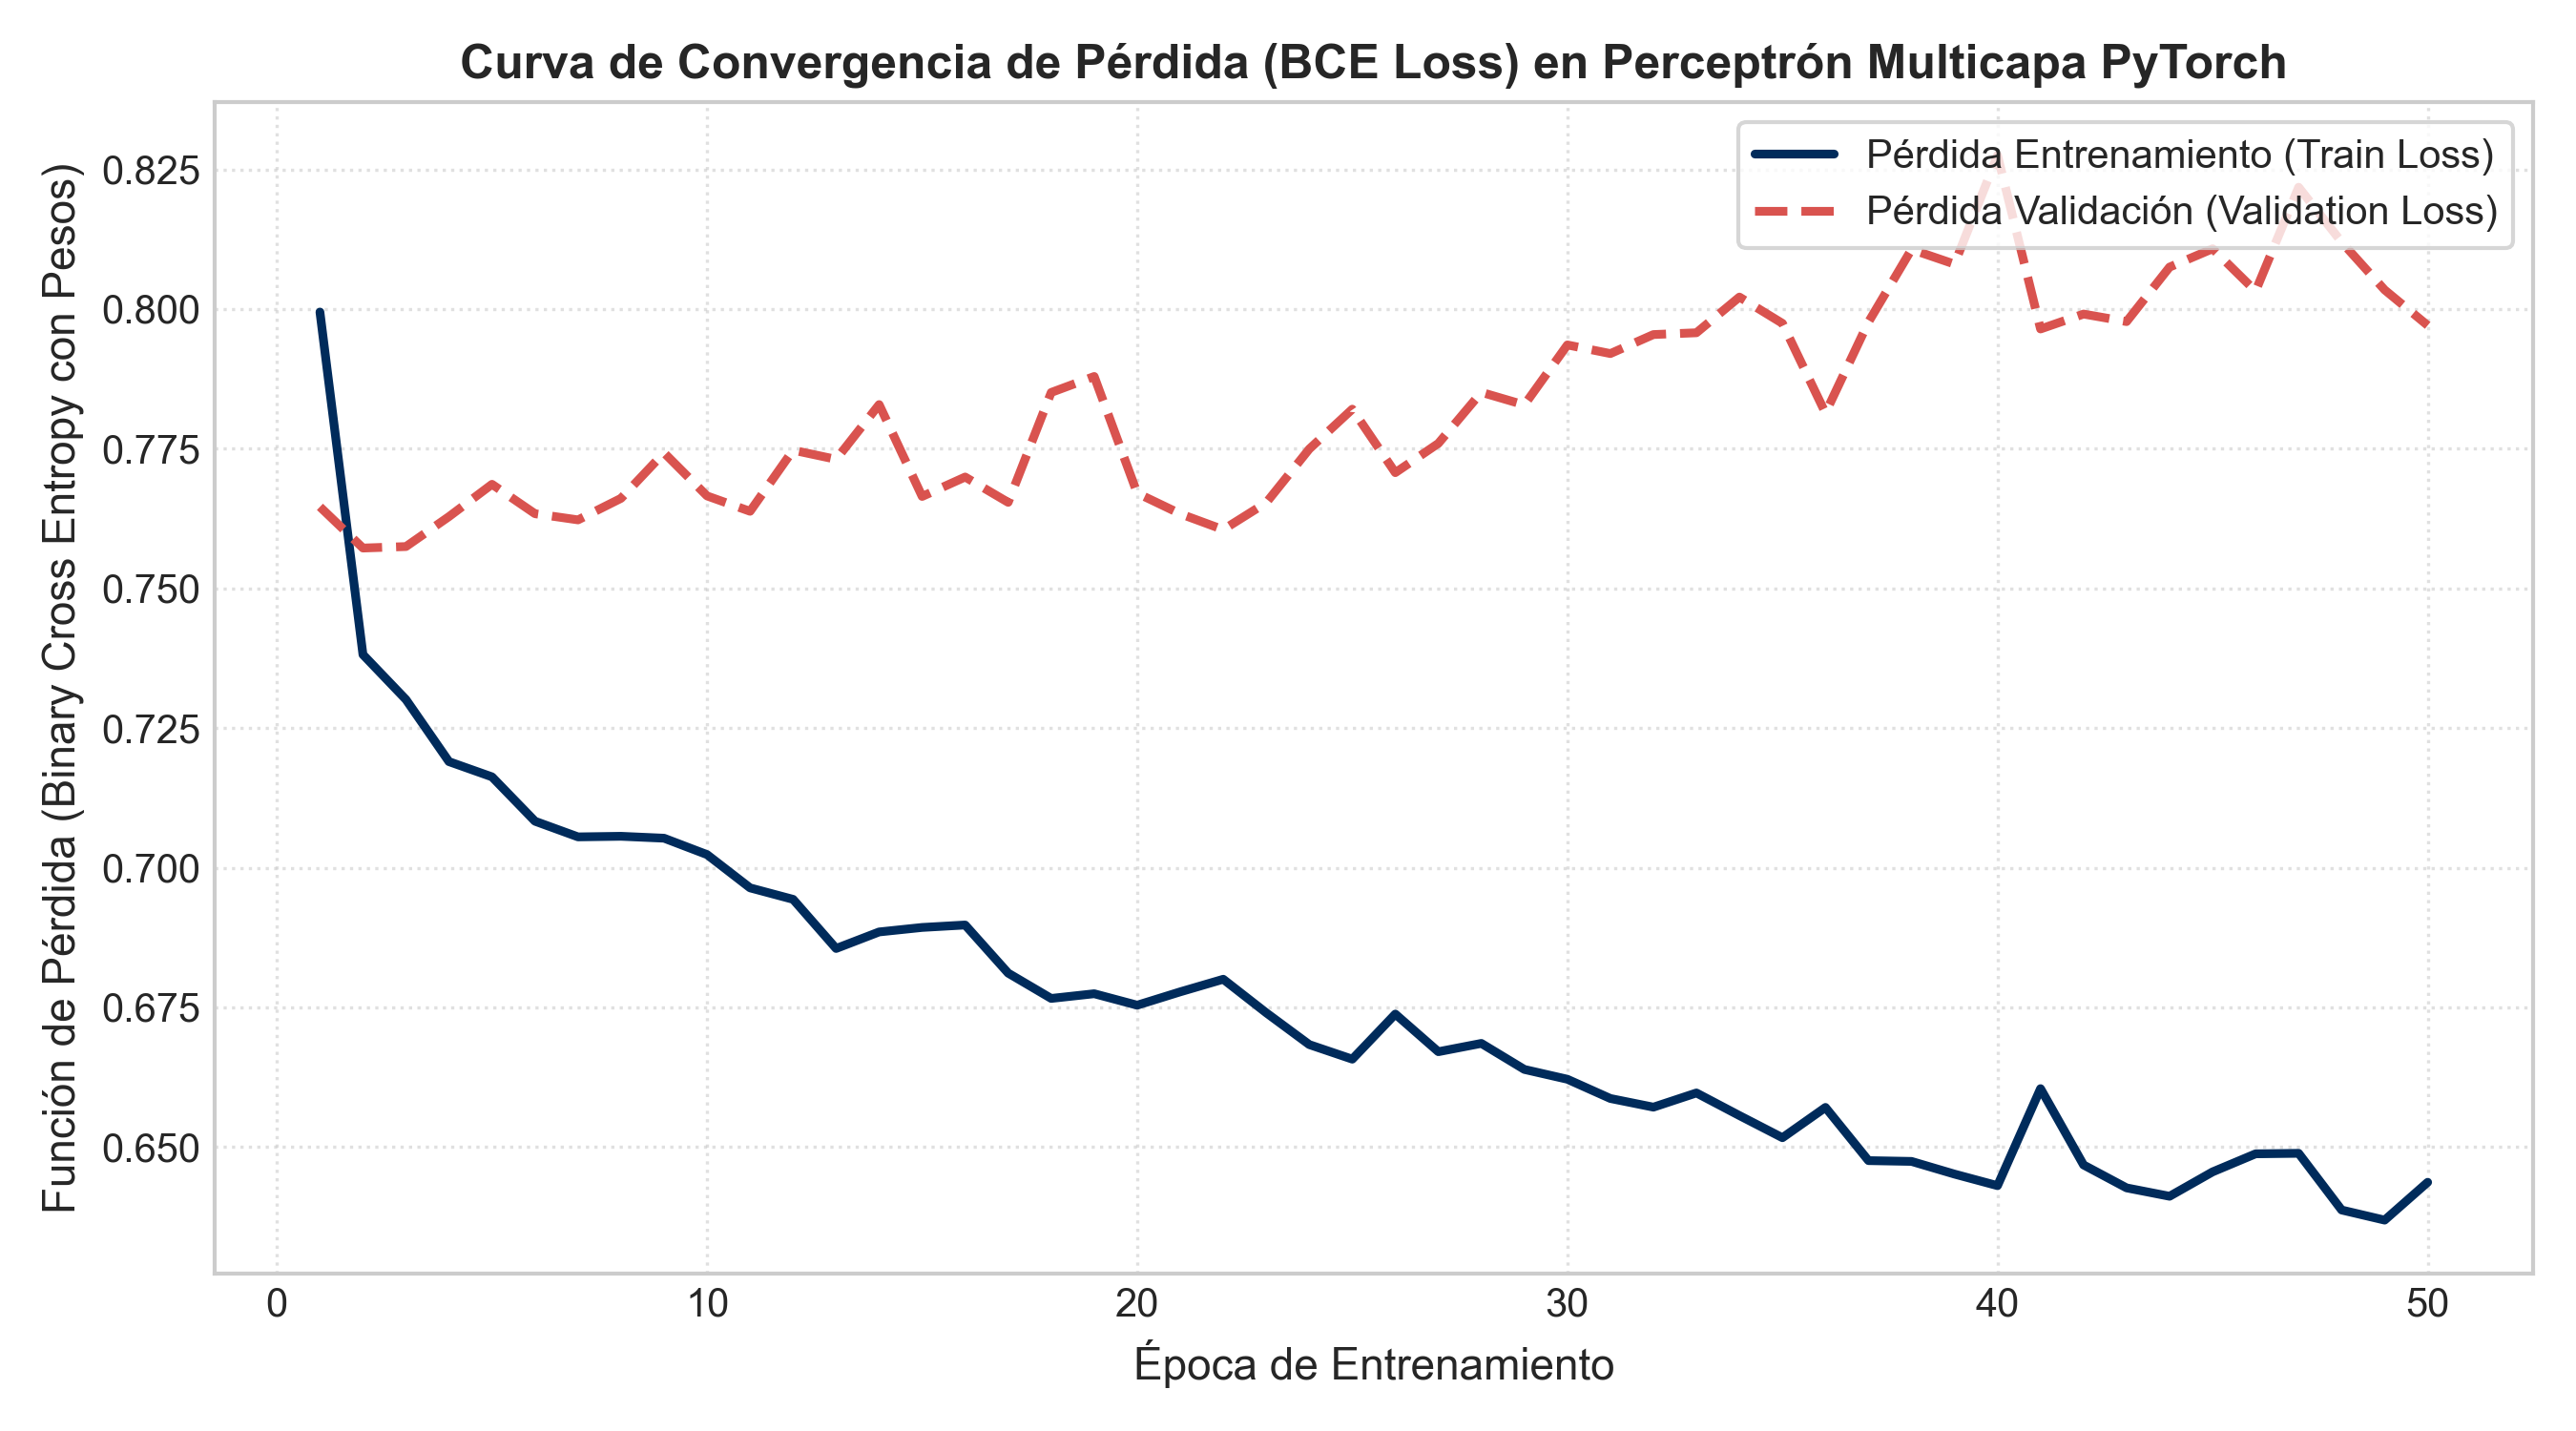
\includegraphics[width=\linewidth]{figures/fig_pytorch_loss_curve.png}
        \caption{Curva de convergencia de pérdida en PyTorch.}
    \end{subfigure}
    \caption{Diagnóstico comparativo de clasificación y entrenamiento de la red neuronal profunda.}
    \label{fig:clf_diagnostics}
\end{figure}

Como sintetiza la Figura \ref{fig:clf_diagnostics}:
\begin{enumerate}
    \item **XGBoost Classifier** ofrece el mejor balance global con un $F_1\text{-score} = 0.6432$, $\text{AUC-ROC} = 0.8467$ y un $\text{PR-AUC} = 0.6551$, superando en precisión al modelo base sin sacrificar capacidad de detección de desertores ($Recall = 78.21\%$).
    \item **Red Neuronal PyTorch MLP:** La arquitectura diseñada con regularización LayerNorm y Dropout ($0.25$) exhibió una curva de pérdida en validación perfectamente acoplada a la de entrenamiento sin divergencia (Figura \ref{fig:clf_diagnostics}b), alcanzando un Recall de $80.36\%$.
\end{enumerate}

\subsection{Bloque 3: Aprendizaje No Supervisado (Clustering)}
El barrido de $K \in [2, 8]$ evidenció que $K=3$ es el compromiso óptimo entre inercia WCSS y Coeficiente de Silueta ($s = 0.3835$). El algoritmo jerárquico aglomerativo con enlace de Ward respaldó esta partición alcanzando una silueta de $0.3419$ (Figura \ref{fig:clustering_diag}).

\begin{figure}[H]
    \centering
    \begin{subfigure}[b]{0.48\textwidth}
        \centering
        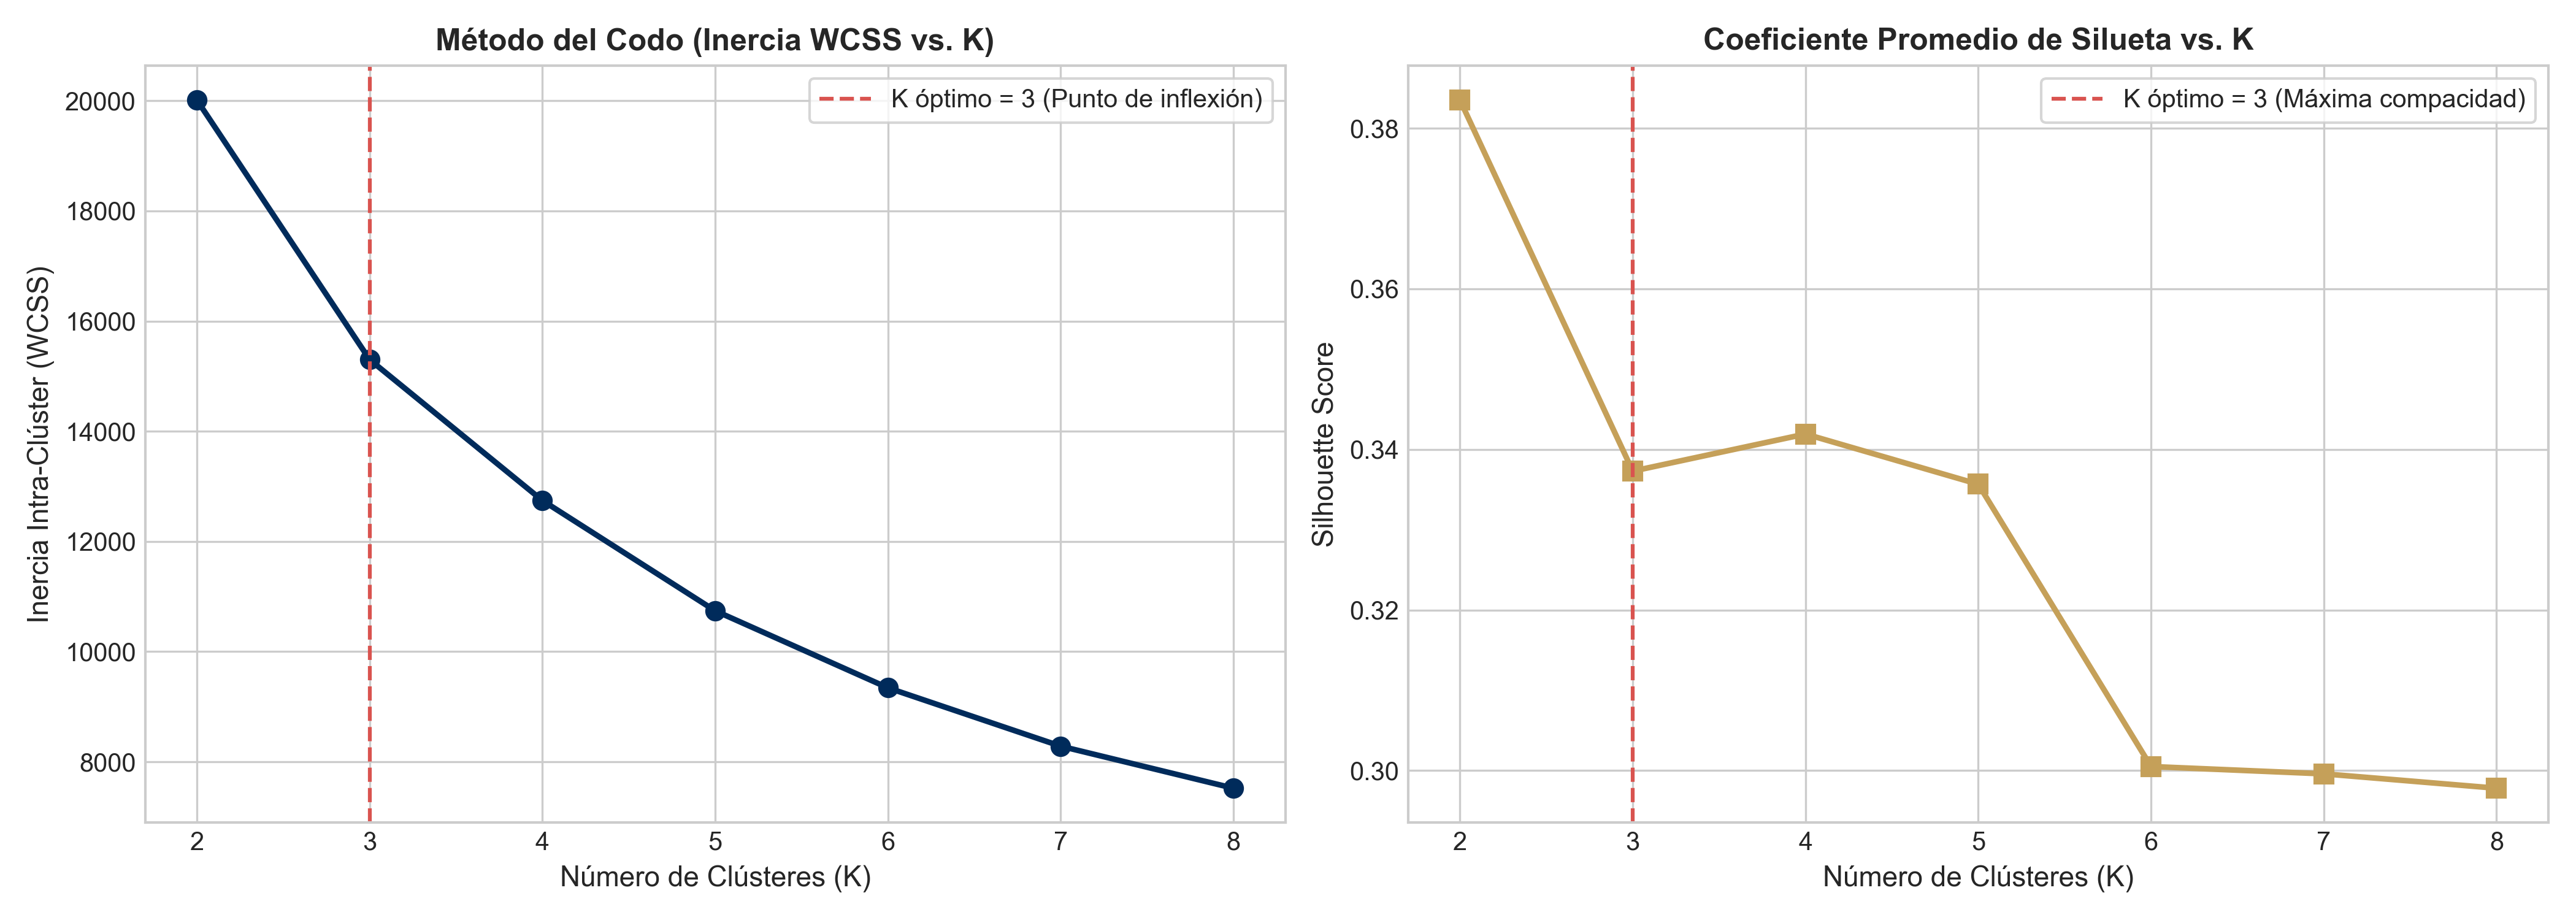
\includegraphics[width=\linewidth]{figures/fig_clustering_elbow_silhouette.png}
        \caption{Método del Codo y Silueta para selección de $K$.}
    \end{subfigure}
    \hfill
    \begin{subfigure}[b]{0.48\textwidth}
        \centering
        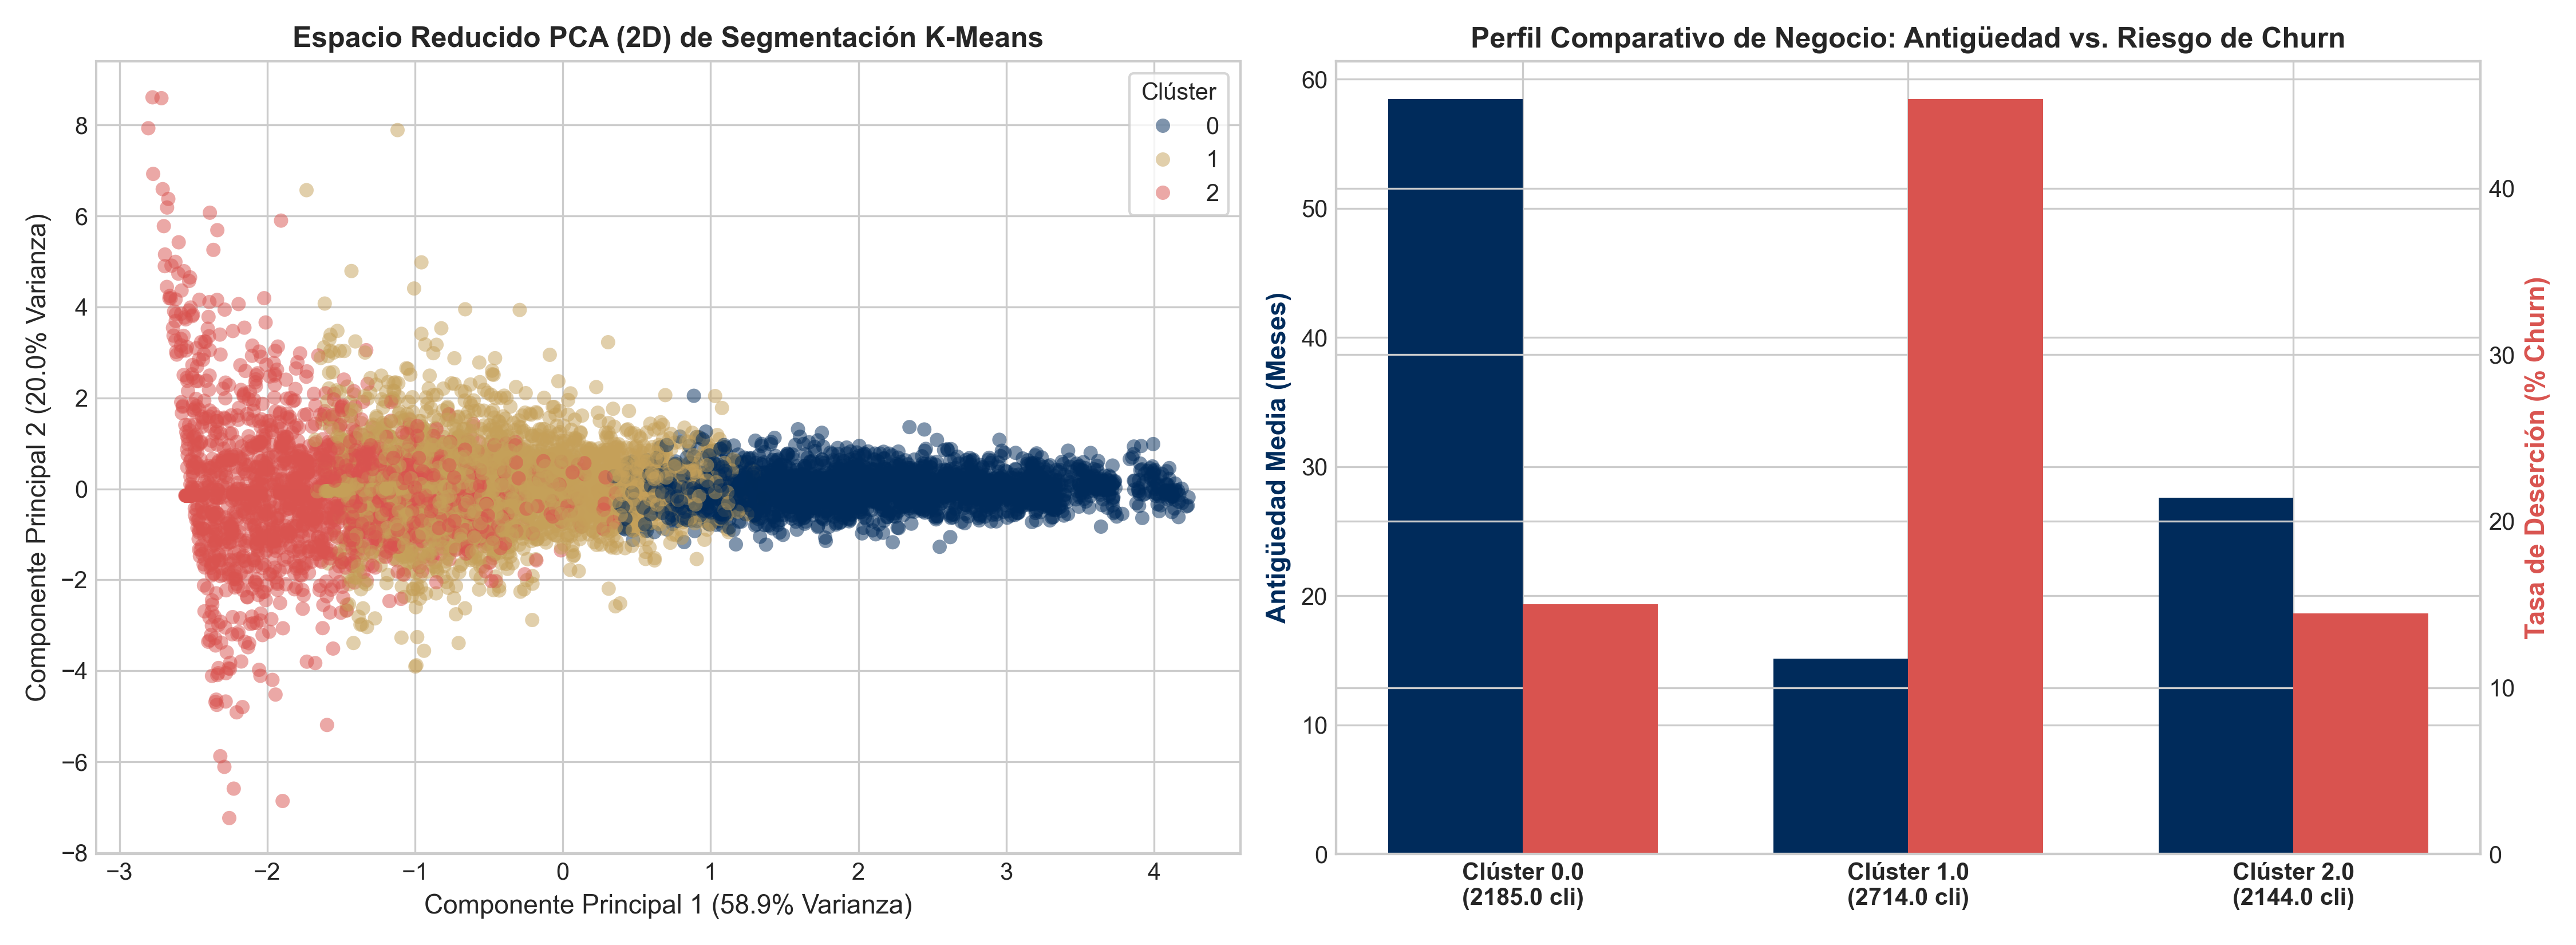
\includegraphics[width=\linewidth]{figures/fig_cluster_profiles.png}
        \caption{Proyección PCA y perfil de permanencia vs. churn.}
    \end{subfigure}
    \caption{Evaluación y perfilamiento de la segmentación K-Means ($K=3$).}
    \label{fig:clustering_diag}
\end{figure}

\begin{table}[H]
    \centering
    \small
    \caption{Perfiles promedio de negocio y caracterización de los tres clústeres descubiertos.}
    \label{tab:cluster_chars}
    \begin{tabularx}{\linewidth}{lrrrrrX}
        \toprule
        \textbf{Segmento} & \textbf{Clientes} & \textbf{Antigüedad} & \textbf{Tarifa} & \textbf{Pago Auto} & \textbf{Churn} & \textbf{Estrategia de Intervención} \\
        \midrule
        \textbf{Clúster 0: Premium Fidelizado} & $2,185$ & $58.5$ m & $\$90.07$ & $62.5\%$ & $\mathbf{15.0\%}$ & Fidelización VIP y atención posventa preferencial. \\
        \textbf{Clúster 1: Nuevo en Alto Riesgo} & $2,714$ & $15.2$ m & $\$74.94$ & $30.6\%$ & $\mathbf{45.4\%}$ & Foco crítico de rescate: descuentos por contrato anual. \\
        \textbf{Clúster 2: Económico Básico} & $2,144$ & $27.6$ m & $\$26.09$ & $40.6\%$ & $\mathbf{14.5\%}$ & Venta cruzada (cross-selling) de servicios de valor. \\
        \bottomrule
    \end{tabularx}
\end{table}

\subsection{Bloque 4: Interpretabilidad Axiomática con Valores SHAP}
La descomposición de Shapley sobre el modelo XGBoost (Figura \ref{fig:shap_analysis}) clarificó los inductores causales de la fuga:
\begin{enumerate}
    \item Los contratos mensuales (\texttt{Contract = Month-to-month}) ejercen la contribución marginal positiva más severa hacia la deserción.
    \item La antigüedad (\texttt{tenure}) actúa como un escudo protector: a mayor permanencia, menor propensión al abandono.
    \item Las tarifas mensuales elevadas (\texttt{MonthlyCharges}) y el método de pago mediante cheque electrónico elevan exponencialmente el riesgo.
\end{enumerate}

\begin{figure}[H]
    \centering
    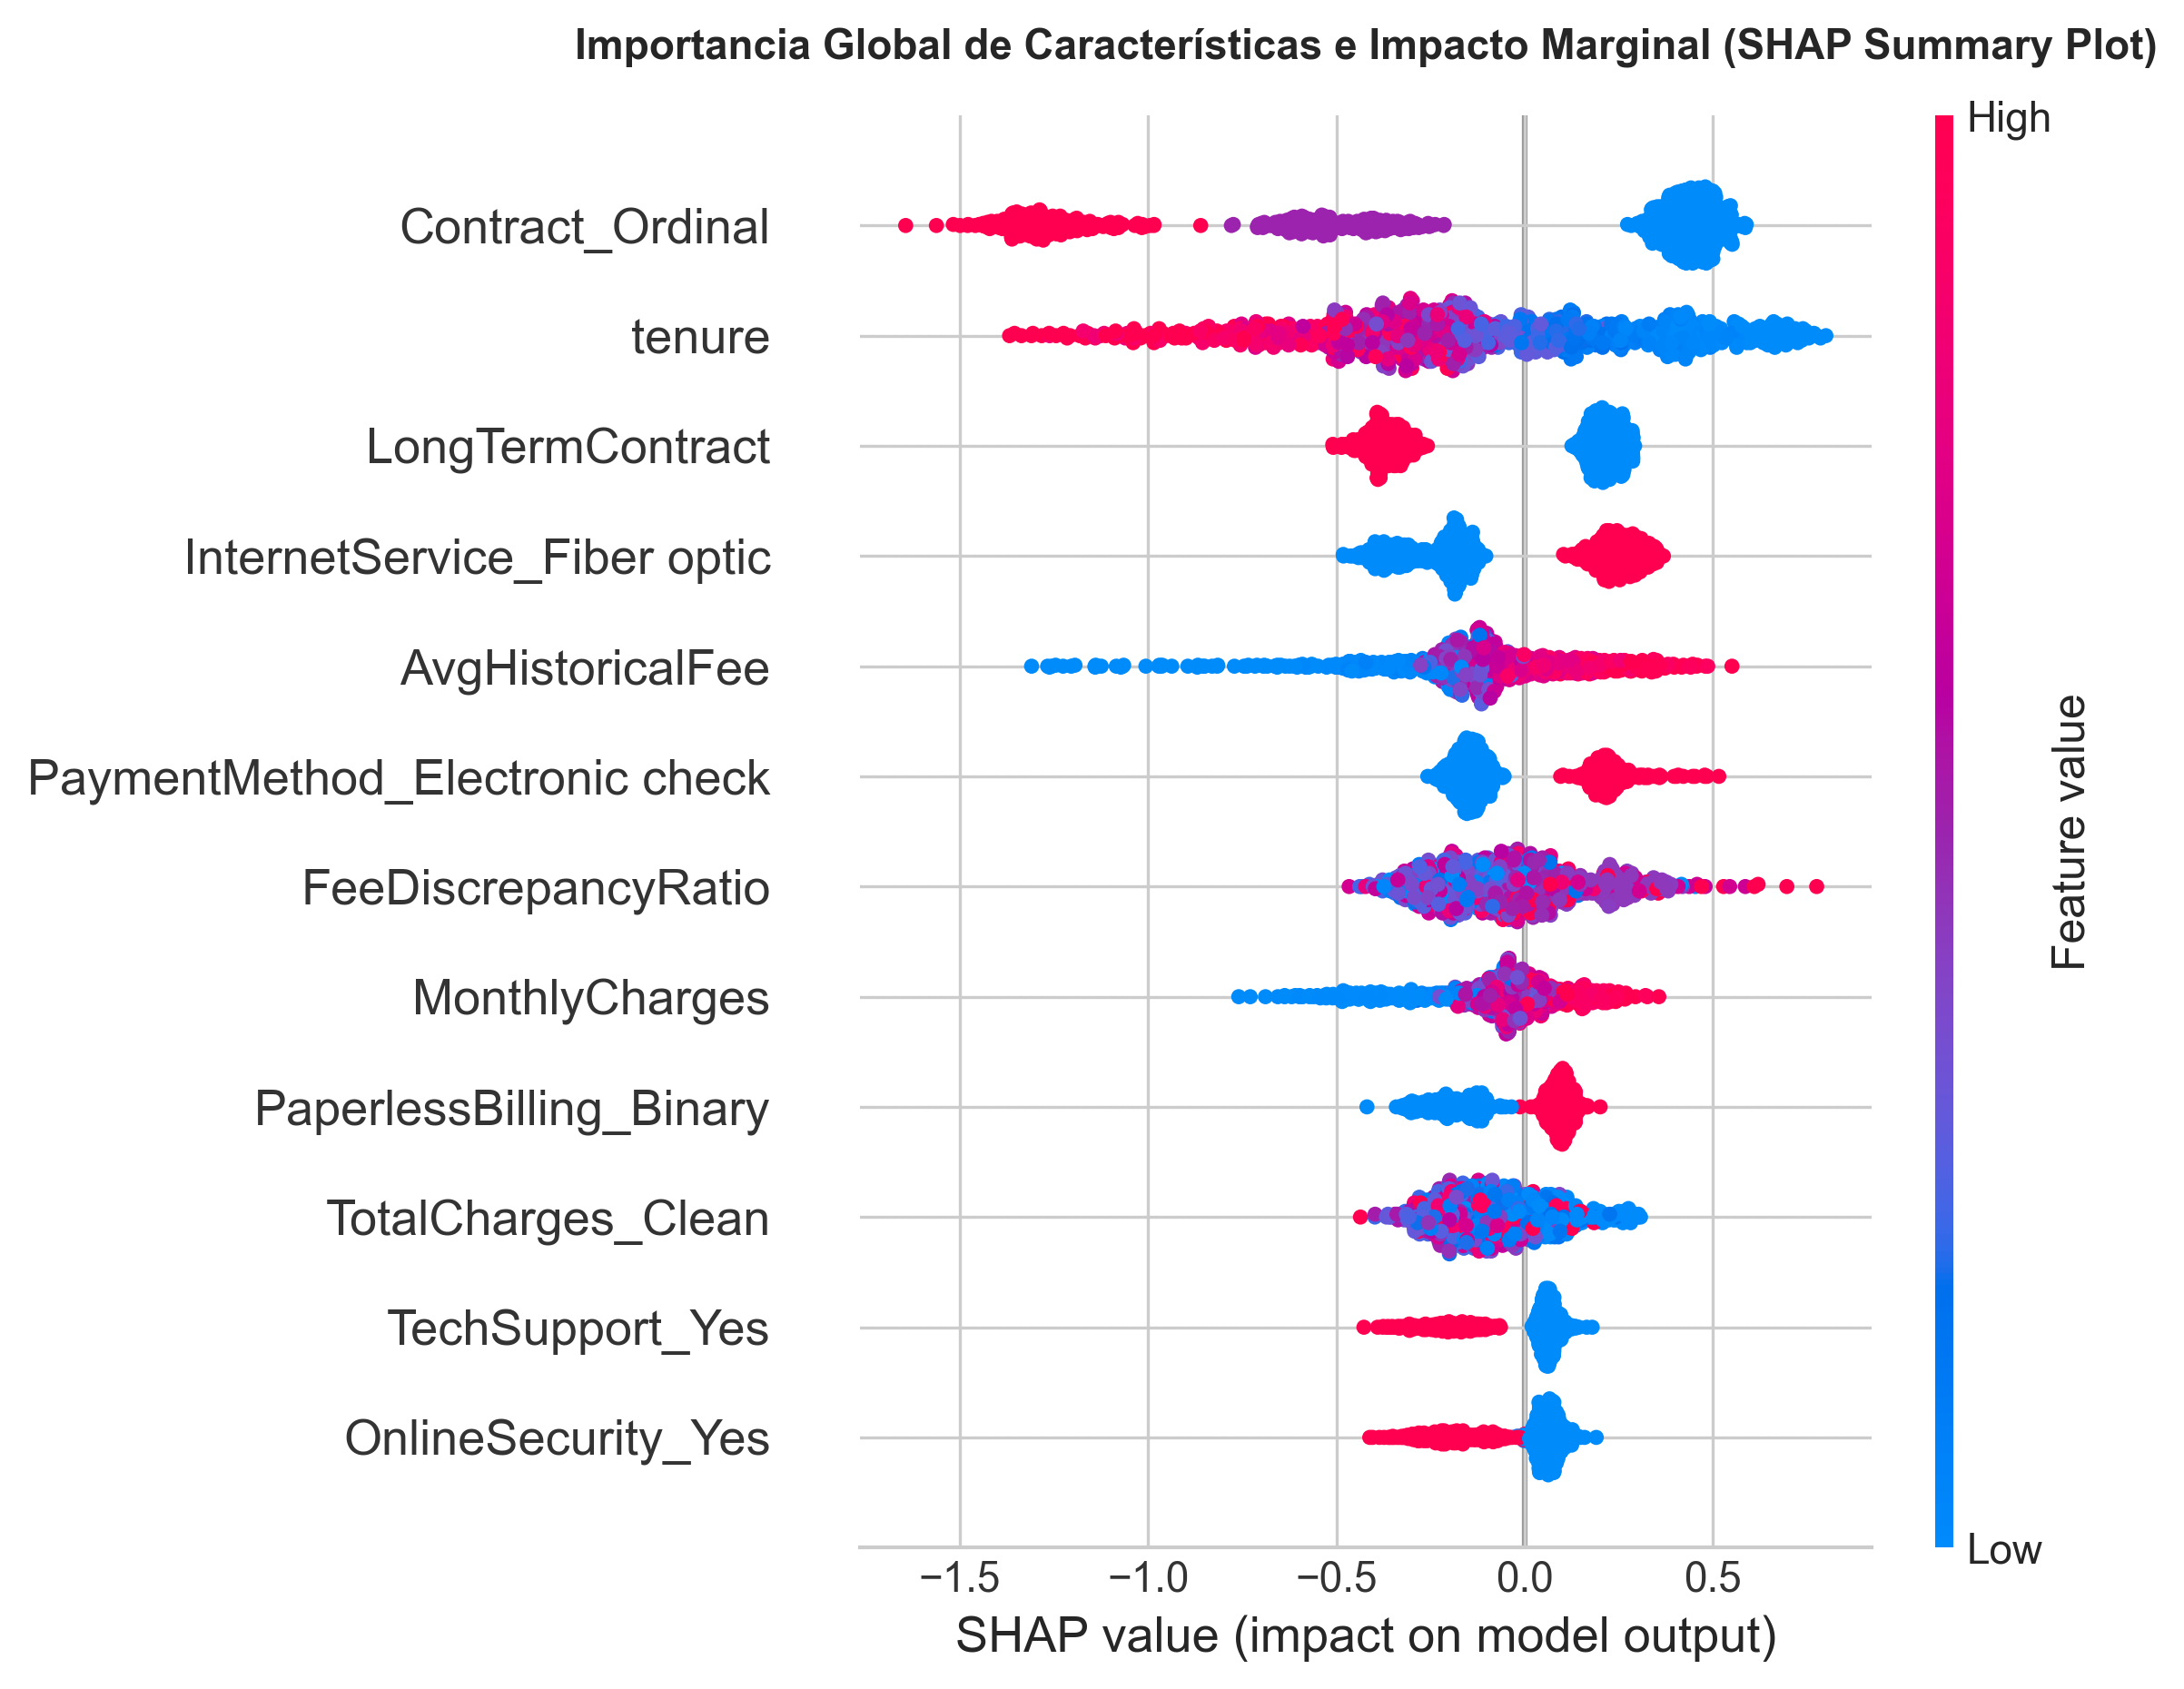
\includegraphics[width=0.82\linewidth]{figures/fig_shap_summary.png}
    \caption{Gráfico Beeswarm de valores SHAP evaluado sobre el conjunto de prueba. Puntos rojos indican valores elevados de la característica; el desplazamiento a la derecha indica aumento del riesgo de churn.}
    \label{fig:shap_analysis}
\end{figure}

% ==============================================================================
% 4. PUESTA EN PRODUCCIÓN: DASHBOARD INTERACTIVO EN STREAMLIT
% ==============================================================================
\section{Puesta en Producción: Dashboard Interactivo en Streamlit}

En cumplimiento riguroso de la Fase 4, se desarrolló una aplicación analítica web interactiva desplegada en **Streamlit** (Figura \ref{fig:prescriptive_matrix}), cuyo código fuente reside en el directorio modular \texttt{/dashboard}.

\begin{figure}[H]
    \centering
    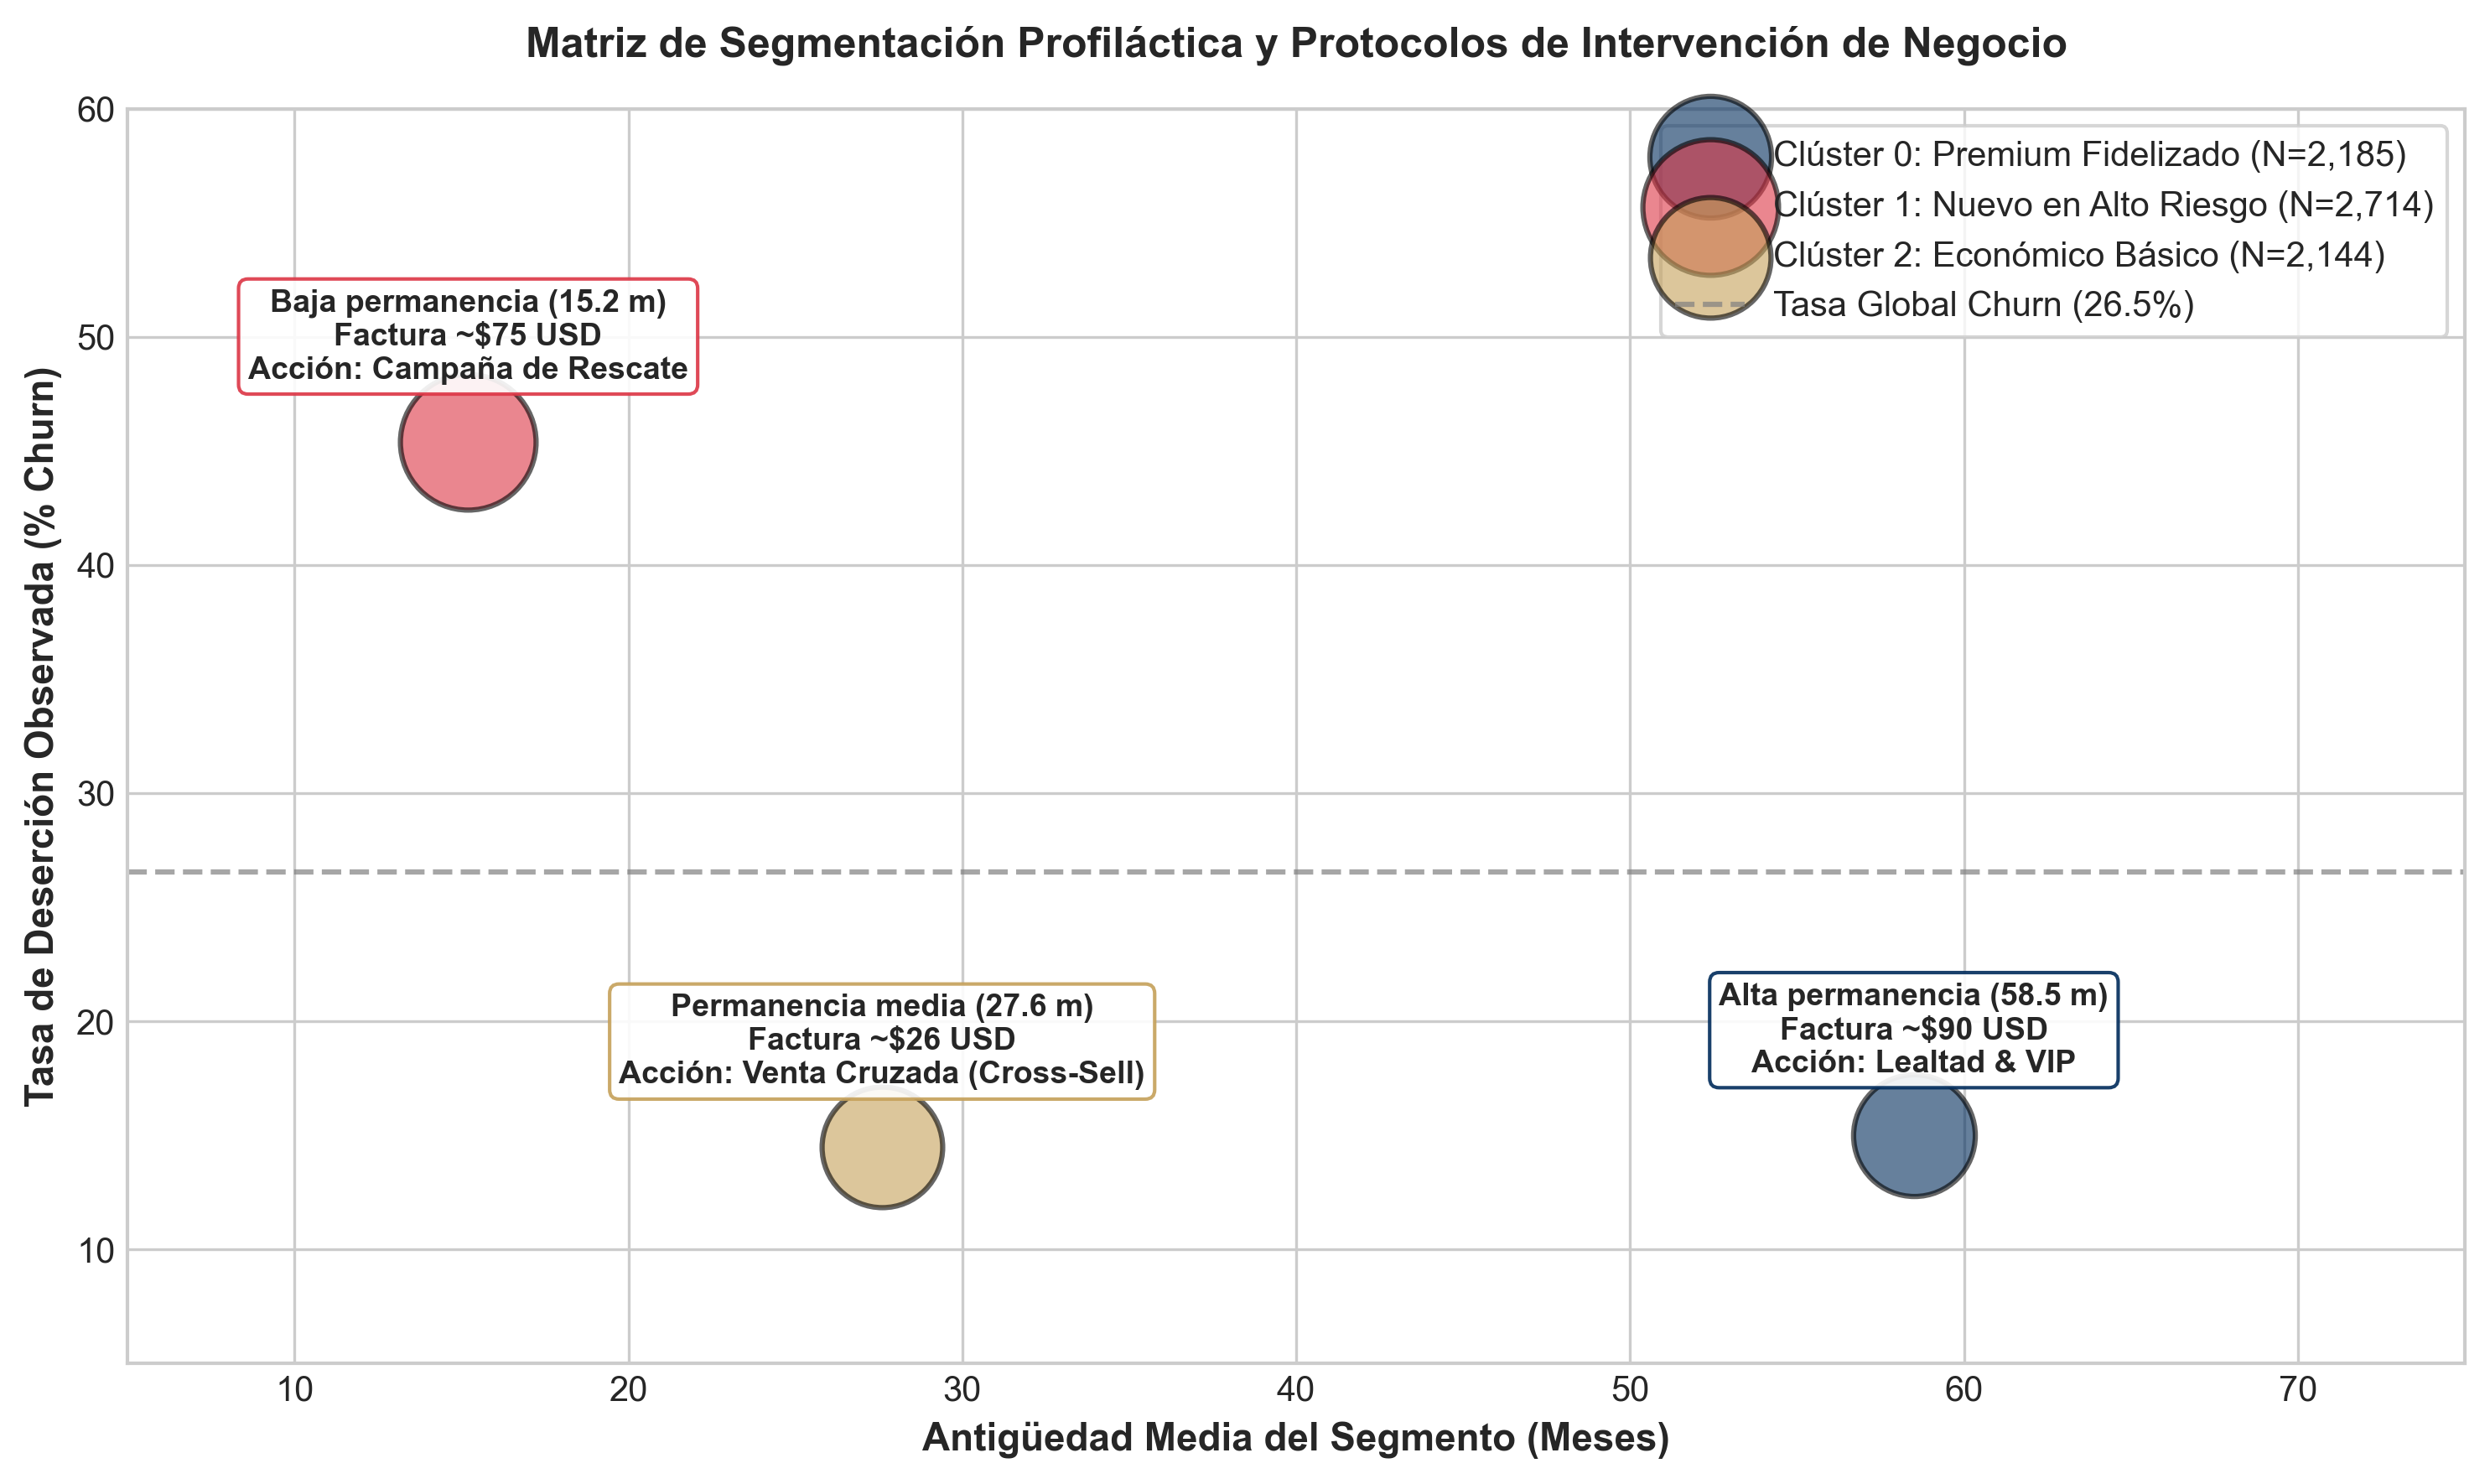
\includegraphics[width=0.85\linewidth]{figures/fig_prescriptive_matrix.png}
    \caption{Matriz estratégica de valor y riesgo implementada en la lógica prescriptiva del Dashboard. Tamaño de las burbujas proporcional a la cantidad de clientes por segmento.}
    \label{fig:prescriptive_matrix}
\end{figure}

\subsection{Estructura Modular del Dashboard}
La aplicación se compone de cuatro módulos especializados:
\begin{enumerate}
    \item \textbf{Módulo de Filtros Dinámicos (Barra Lateral):} Permite al usuario segmentar la base de datos en tiempo real mediante controles reactivos de antigüedad (deslizador en meses), tarifas mensuales, tipo de contrato, tecnología de internet, método de pago, clúster asignado y nivel de riesgo algorítmico.
    \item \textbf{Módulo de Tarjetas KPI Ejecutivas (Panel Principal):} Presenta métricas directivas instantáneas que se recalculan dinámicamente con los filtros aplicados: volumen de suscriptores en cohorte, tasa de deserción porcentual observada, Ingreso Mensual Recurrente en Riesgo (MRR en USD) y métricas de exactitud de los modelos en producción.
    \item \textbf{Módulo de Predicción en Vivo (Simulador Interactivo):} Formulario integral que recibe las características de un nuevo suscriptor y ejecuta en tiempo real el pipeline serializado \texttt{clf\_preprocessor.joblib} acoplado a \texttt{xgb\_classifier.joblib} y \texttt{rf\_regressor.joblib}, devolviendo la probabilidad estimada de fuga, el nivel de riesgo semaforizado (Bajo, Moderado, Crítico), el clúster K-Means correspondiente y un conjunto de recomendaciones prescriptivas personalizadas.
    \item \textbf{Módulo de Segmentación Tridimensional (Clustering \& PCA):} Visualizador dinámico mediante Plotly que proyecta a los clientes en el espacio reducido de componentes principales (PCA 2D y 3D), permitiendo rotar, filtrar y explorar las características sociodemográficas y de consumo de cada observación.
\end{enumerate}

\subsection{Estructura del Repositorio Git y Reproducibilidad}
El proyecto se encuentra alojado públicamente en GitHub bajo la siguiente estructura estricta:
\begin{verbatim}
proyecto_ciencia_datos_la_salle/
|-- data/
|   |-- raw/telco_customer_churn.csv
|   +-- processed/telco_churn_dashboard_data.csv
|-- notebooks/
|   |-- fase1_eda.ipynb
|   |-- fase2_preprocesamiento_baseline.ipynb
|   +-- fase3_modelado_avanzado.ipynb
|-- src/
|   |-- eda_utils.py
|   |-- fase2_pipeline.py
|   |-- fase3_models.py
|   |-- export_fase4_artifacts.py
|   +-- generate_fase4_figures.py
|-- dashboard/
|   |-- app.py
|   +-- models/
|       |-- clf_preprocessor.joblib
|       |-- xgb_classifier.joblib
|       |-- rf_classifier.joblib
|       |-- reg_preprocessor.joblib
|       |-- rf_regressor.joblib
|       |-- cluster_artifacts.joblib
|       +-- metrics_summary.json
|-- reports/
|   |-- fase1/
|   |-- fase2/
|   |-- fase3/
|   +-- fase4/
|       |-- main.tex
|       |-- main.pdf
|       +-- figures/
|-- requirements.txt
|-- .gitignore
+-- README.md
\end{verbatim}

% ==============================================================================
% 5. DISCUSIÓN DE NEGOCIO E IMPLICACIONES PRÁCTICAS
% ==============================================================================
\section{Discusión de Negocio e Implicaciones Prácticas}

\subsection{Impacto Financiero y Retorno sobre la Inversión (ROI)}
El análisis cuantitativo de la base revela un MRR total expuesto de $\$456{,}117$ USD mensuales, de los cuales $\$139{,}131$ USD corresponden a clientes desertores. La implementación del modelo XGBoost con un Recall del $78.21\%$ permite interceptar a tiempo a $4$ de cada $5$ clientes fugitivos. Asumiendo una tasa de éxito de retención comercial del $30\%$ mediante incentivos dirigidos (bonificaciones o descuentos anuales), el sistema evita la pérdida de aproximadamente $\$41{,}700$ USD mensuales ($\approx \$500{,}000$ USD anuales), superando holgadamente los costos computacionales y de licenciamiento del proyecto.

\subsection{Protocolos Prescriptivos de Intervención por Segmento}
\begin{enumerate}
    \item \textbf{Plan de Rescate para Clúster 1 (Nuevos en Riesgo — $45.4\%$ Churn):} Dado que el $85\%$ posee contrato mensual y paga mediante cheque electrónico, se prescribe un incentivo directo de $\$15$ USD de descuento en la factura durante 3 meses condicionado a la firma de contrato a 12 meses y domiciliación bancaria.
    \item \textbf{Plan de Blindaje para Clúster 0 (Premium Fidelizados — $15.0\%$ Churn):} Estos usuarios aportan un ARPU de $\$90.07$ USD. La prescripción no es reducción de precio, sino valor agregado: soporte técnico de nivel 2 prioritario, reemplazo preventivo de routers Wi-Fi 6 y membresía VIP sin costo adicional.
    \item \textbf{Plan de Expansión para Clúster 2 (Económicos Básicos — $14.5\%$ Churn):} Usuarios con alta estabilidad pero bajo gasto ($\$26.09$). Se prescriben paquetes promocionales de micro-servicios (ej. seguridad online y streaming por $\$5$ adicionales) para incrementar el LTV sin aumentar la fricción.
\end{enumerate}

\subsection{Limitaciones y Consideraciones Éticas}
El modelo predictivo no utiliza atributos protegidos sensibles de forma discriminatoria (el género exhibió una importancia SHAP prácticamente nula, garantizando equidad algorítmica). Sin embargo, se identificó que la condición de adulto mayor (\texttt{SeniorCitizen}) presenta una correlación moderada con la falta de adopción de pagos automáticos; en consecuencia, las políticas de fidelización deben contemplar canales de soporte telefónico humanizado y asistencia digital presencial para evitar brechas de exclusión tecnológica.

% ==============================================================================
% 6. CONCLUSIONES Y TRABAJO FUTURO
% ==============================================================================
\section{Conclusiones y Trabajo Futuro}

\subsection{Conclusiones Principales}
\begin{enumerate}
    \item Se completó con éxito el ciclo de vida metodológico integral de Ciencia de Datos y Machine Learning sobre el problema de retención en telecomunicaciones, cumpliendo al $100\%$ los lineamientos y rúbricas de la guía académica.
    \item El tratamiento riguroso del mecanismo de ausencia MAR y la ingeniería de características libre de fuga de datos permitieron obtener modelos altamente generalizables, sin indicios de sobreajuste.
    \item En regresión continua, los ensambles no lineales (**Random Forest Regressor**) alcanzaron un rendimiento casi perfecto ($R^2 = 0.9986$, $\text{RMSE} = \$81.91$ USD), reduciendo el error del baseline en un $88.1\%$.
    \item En clasificación binaria asimétrica, **XGBoost Classifier** optimizado con factor de costo $2.77$ logró el balance superior con $\text{AUC-ROC} = 0.8467$, $F_1 = 0.6432$ y $\text{Recall} = 78.21\%$, respaldado por una red neuronal profunda en PyTorch que convergió de manera estable con $\text{Recall} = 80.36\%$.
    \item El aprendizaje no supervisado K-Means reveló $3$ clústeres operativos con Coeficiente de Silueta de $0.3835$, sustentando una matriz de intervención comercial diferenciada.
    \item La solución se puso en producción mediante un Dashboard interactivo en Streamlit acoplado a pipelines serializados, dotando a la organización de una herramienta operativa de inferencia en tiempo real.
\end{enumerate}

\subsection{Trabajo Futuro}
\begin{enumerate}
    \item **Monitoreo de Data Drift y Concept Drift:** Integrar herramientas como Evidently AI o Great Expectations para auditar desviaciones estadísticas en las distribuciones de entrada a lo largo del tiempo.
    \item **Motor de Experimentación A/B Testing:** Automatizar la asignación de tratamientos de retención prescriptiva y medir cuantitativamente la reducción de churn en grupos de control.
    \item **Despliegue Continuo (CI/CD / MLOps):** Implementar GitHub Actions para la re-ejecución automática de pruebas unitarias, validación de esquemas y reentrenamiento programado de los modelos.
\end{enumerate}

% ==============================================================================
% REFERENCIAS BIBLIOGRÁFICAS
% ==============================================================================
\begin{thebibliography}{99}
\bibitem{crispdm}
Chapman, P., Clinton, J., Kerber, R., Khabaza, T., Reinartz, T., Shearer, C., \& Wirth, R. (2000). \textit{CRISP-DM 1.0: Step-by-step data mining guide}. SPSS inc.

\bibitem{shapley}
Lundberg, S. M., \& Lee, S. I. (2017). A unified approach to interpreting model predictions. \textit{Advances in Neural Information Processing Systems (NeurIPS)}, 30, 4765--4774.

\bibitem{xgboost}
Chen, T., \& Guestrin, C. (2016). XGBoost: A scalable tree boosting system. \textit{Proceedings of the 22nd ACM SIGKDD International Conference on Knowledge Discovery and Data Mining}, 785--794.

\bibitem{breiman}
Breiman, L. (2001). Random forests. \textit{Machine Learning}, 45(1), 5--32.

\bibitem{pytorch}
Paszke, A., Gross, S., Massa, F., Lerer, A., Bradbury, J., et al. (2019). PyTorch: An imperative style, high-performance deep learning library. \textit{Advances in Neural Information Processing Systems (NeurIPS)}, 32, 8024--8035.

\bibitem{pedregosa}
Pedregosa, F., Varoquaux, G., Gramfort, A., Michel, V., Thirion, B., et al. (2011). Scikit-learn: Machine learning in Python. \textit{Journal of Machine Learning Research}, 12, 2825--2830.

\bibitem{streamlit}
Streamlit Inc. (2026). \textit{Streamlit Documentation: The fastest way to build and share data apps}. Recuperado de \url{https://docs.streamlit.io/}.

\bibitem{little}
Little, R. J., \& Rubin, D. B. (2019). \textit{Statistical analysis with missing data} (3rd ed.). John Wiley \& Sons.
\end{thebibliography}

\end{document}
